\chapter{Capacitively Coupled Pixel Detectors for the CLIC Vertex Detector}
\label{chap:theory}

\chapterquote{There, sir! that is the perfection of vessels!}
{Jules Verne, 1828--1905}

\section{Introduction}
Successful identification of heavy-flavour quarks and tau-leptons relies upon precise reconstruction of the secondary displaced vertices produced in the decay of these particles as well as accurate association of the daughter tracks to those vertices.  To achieve this for the CLIC experiment very high spatial resolution, of approximately 3 {\mu}m and good geometric coverage extending to low $\theta$ values are essential.  The vertex detector must also have a low material budget, less than 0.2 $\text{X}_{0}$ per layer, as to not impact the performance of the other sub detectors and a low occupancy, aided by time-tagging to an accuracy of 10 ns, to counteract the high beam-induced backgrounds found near the impact point.  

There are no commercially available technology options that fulfil all the criteria for the vertex detector, which had led the CLIC experiment to consider a variety of new technology options.  The focus of this chapter is the use of high voltage complementary metal-oxide-semiconductor (HV-CMOS) active sensors coupled to a separate readout ASIC for the CLIC vertex detector.  

% Active sensor does something to signal when recorded, passive just records signel.  HV-CMOS is active as there's an amplification of signal step.

\subsection{HV-CMOS}
There are two classifications for pixel detectors; hybrid detectors where a passive sensor is bump-bonded to a separate readout chip and fully integrated where the collection diode is built upon the same wafer as the readout circuitry.  Both of these technology options find the CLIC experimental conditions extremely challenging.  Hybrid technologies struggle to achieved both the radiation tolerance and the functionality in the readout circuitry, while fully integrated circuits have too slow readout times due to limitations on the applied bias voltage.  

HV-CMOS is adapted to the CLIC experimental conditions as the n-MOS and p-MOS transistors forming the integrated amplifier (or generic in-pixel logic operations in general) for collecting the signal are embedded within a deep n-well, as shown in figure \ref{fig:hvcmos}.  This acts as both the collection diode as well as providing shielding to the circuitry from the beam induced radiation.  With the integrated circuitry shielded from the p-substrate it becomes possible to apply a large bias voltage to the substrate to widen the depletion region meaning that the main part of any signal deposited in the detector will be transferred via drift as opposed to diffusion, which provides the fast readout times required by the CLIC experiment.  

\begin{figure}
\centering
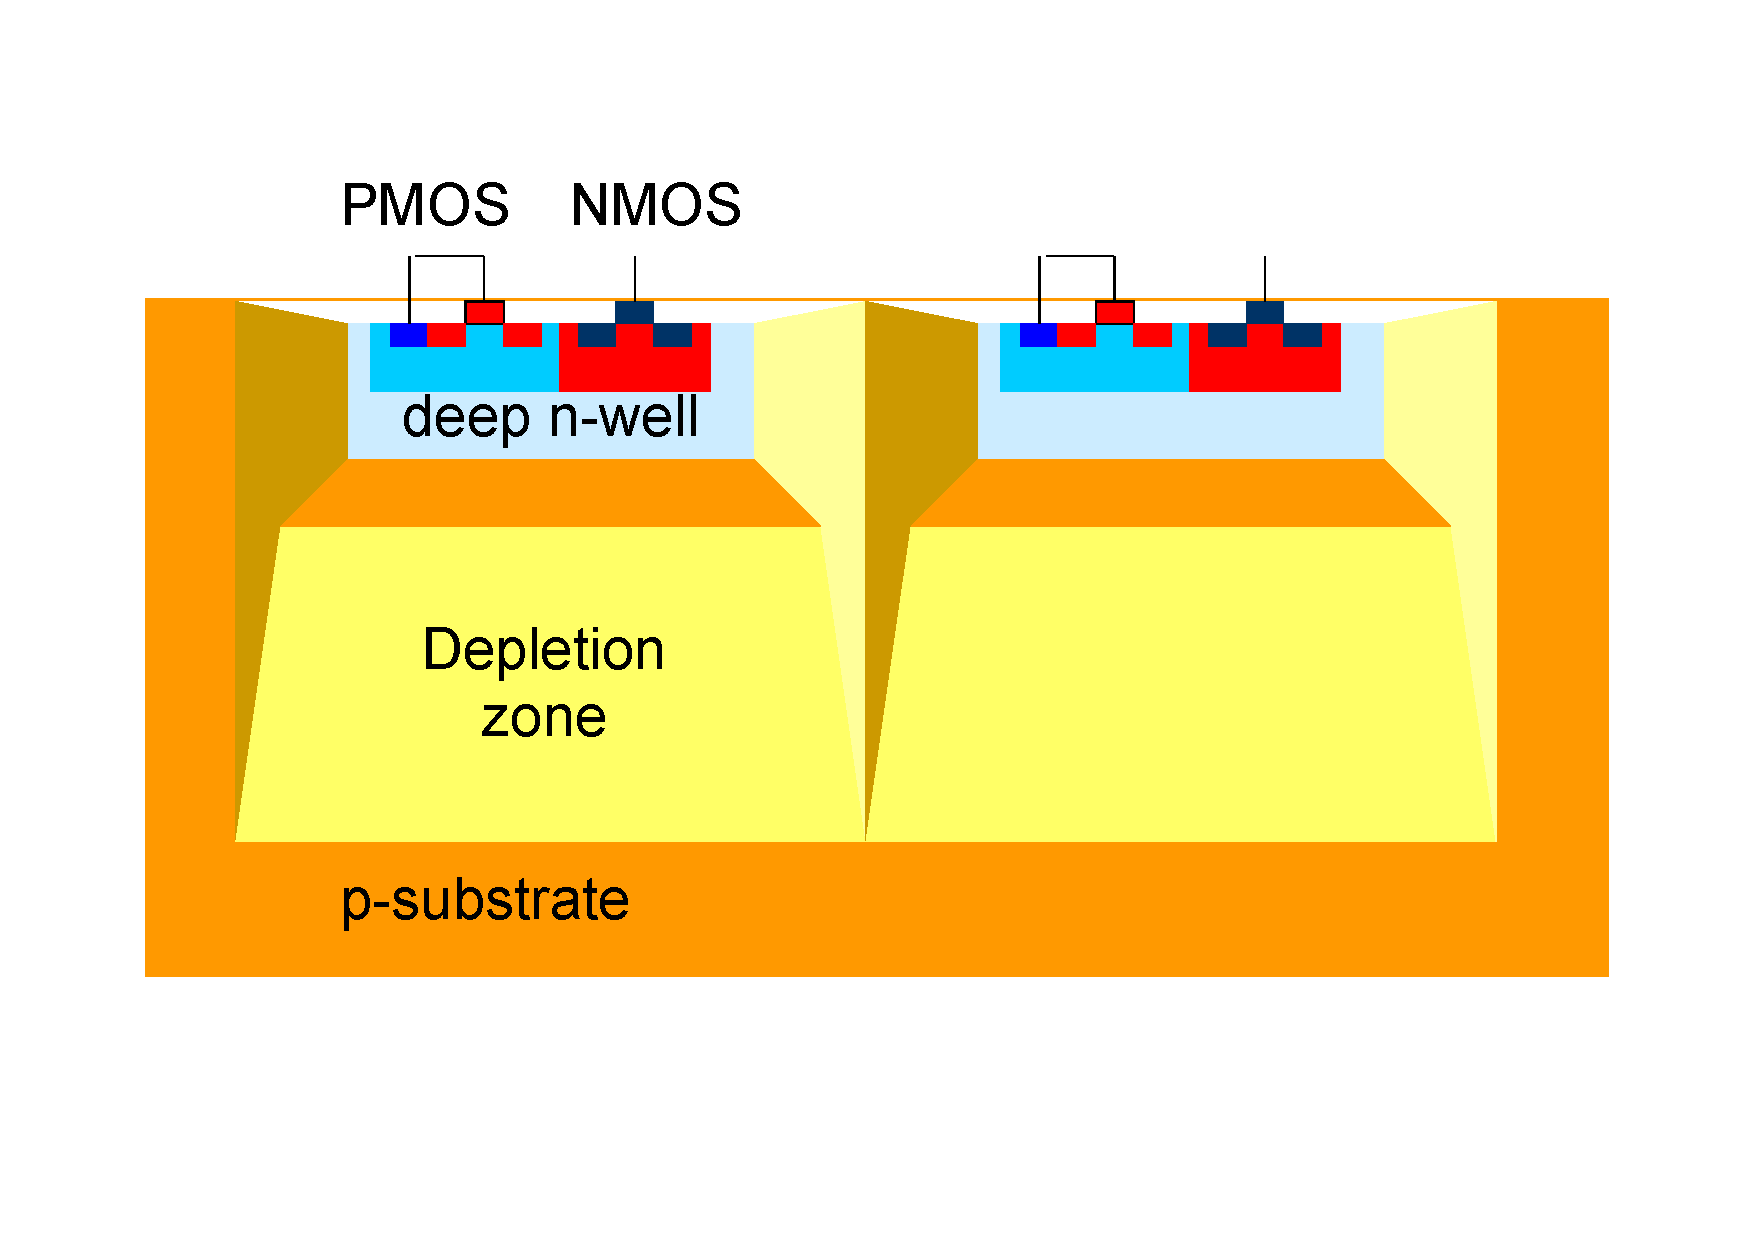
\includegraphics[width=0.75\textwidth]{CLICdpVertex/Plots/HV-CMOSDiagram.pdf}
\caption[HV-CMOS diagram.]{HV-CMOS diagram.}
\label{fig:hvcmos}
\end{figure}

HV-CMOS devices are strong candidates for the CLIC vertex detector, however, they do have limitations such as noise from interference between the n and p doped wells of the n-MOS and p-MOS transistors that sit within the deep n well.  This noise will grow with the number of n-MOS and p-MOS devices on the wafer and so ultimately restricts the complexity of the in-pixel operations that can be performed.  There are also topological difficulties such as the difficulty of applying the CMOS process to all sizes and the fact that the deep n well does not occupy the full space of the pixel.  

To minimise the material budget for the vertex detector, the pixels used are designed to be as thin as possible.  This means the signal from the HV-CMOS will be small as the depletion region will be thin.  To counter this, in-pixel signal amplification was applied to the HV-CMOS devices, as shown in figure \ref{fig:ccpdandclicpix}.  This increases the signal going to the readout ASIC, which also counteracts the intrinsically small capacitance between the HV-CMOS and readout ASIC.

\begin{figure}
\centering
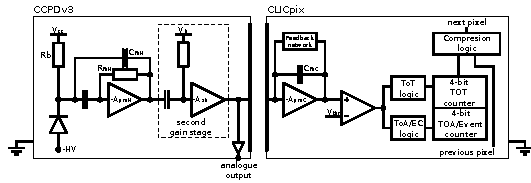
\includegraphics[width=1.0\textwidth]{CLICdpVertex/Plots/schematic.pdf}
\caption[Schematic of CCPDv3 and CLICpix pixels.]{Schematic of CCPDv3 and CLICpix pixels.}
\label{fig:ccpdandclicpix}
\end{figure}

\subsection{CLICpix}
The readout ASIC in this study is the CLICpix, which is a charge integrating amplifier connected to a discriminator as shown in figure \ref{fig:ccpdandclicpix}.  The output to this discriminator is then used as the input for further logic operations that record the magnitude, using a Time over Threshold (ToT) measurement, and time of arrival of the collected charge.

\subsection{Capacitive Coupling}
Solder bump-bonding is the typical method that is used for connecting active pixel sensors to the readout ASIC, however, the solder adds to the thickness of the sensor significantly as well as raising the cost.  A viable alternative to this procedure is the replacement of the bump-bonding with a thin uniform layer of glue that forms a capacitive connection between the active pixel and readout ASIC.  The mechanical tolerances on the alignment of the active pixel sensor and readout ASIC when applying this glueing procedure are the focus of this study.  

\section{Construction}
While replacing solder bump-bonding with a thin layer of glue in the construction of the sensors for the vertex detector offers benefits, such as reductions in the material budget and cost, the manufacturing procedure could lead to misalignments between the active pixel sensor and the readout ASIC.  To determine the impact of these misalignments a number of sensors were constructed using the gluing procedure that contained offsets between the HV-CMOS and CLICpix, as shown in figure \ref{fig:alignment}.  A table \ref{table:alignment} contains a summary of all the samples used in this study.

\begin{figure}
\centering
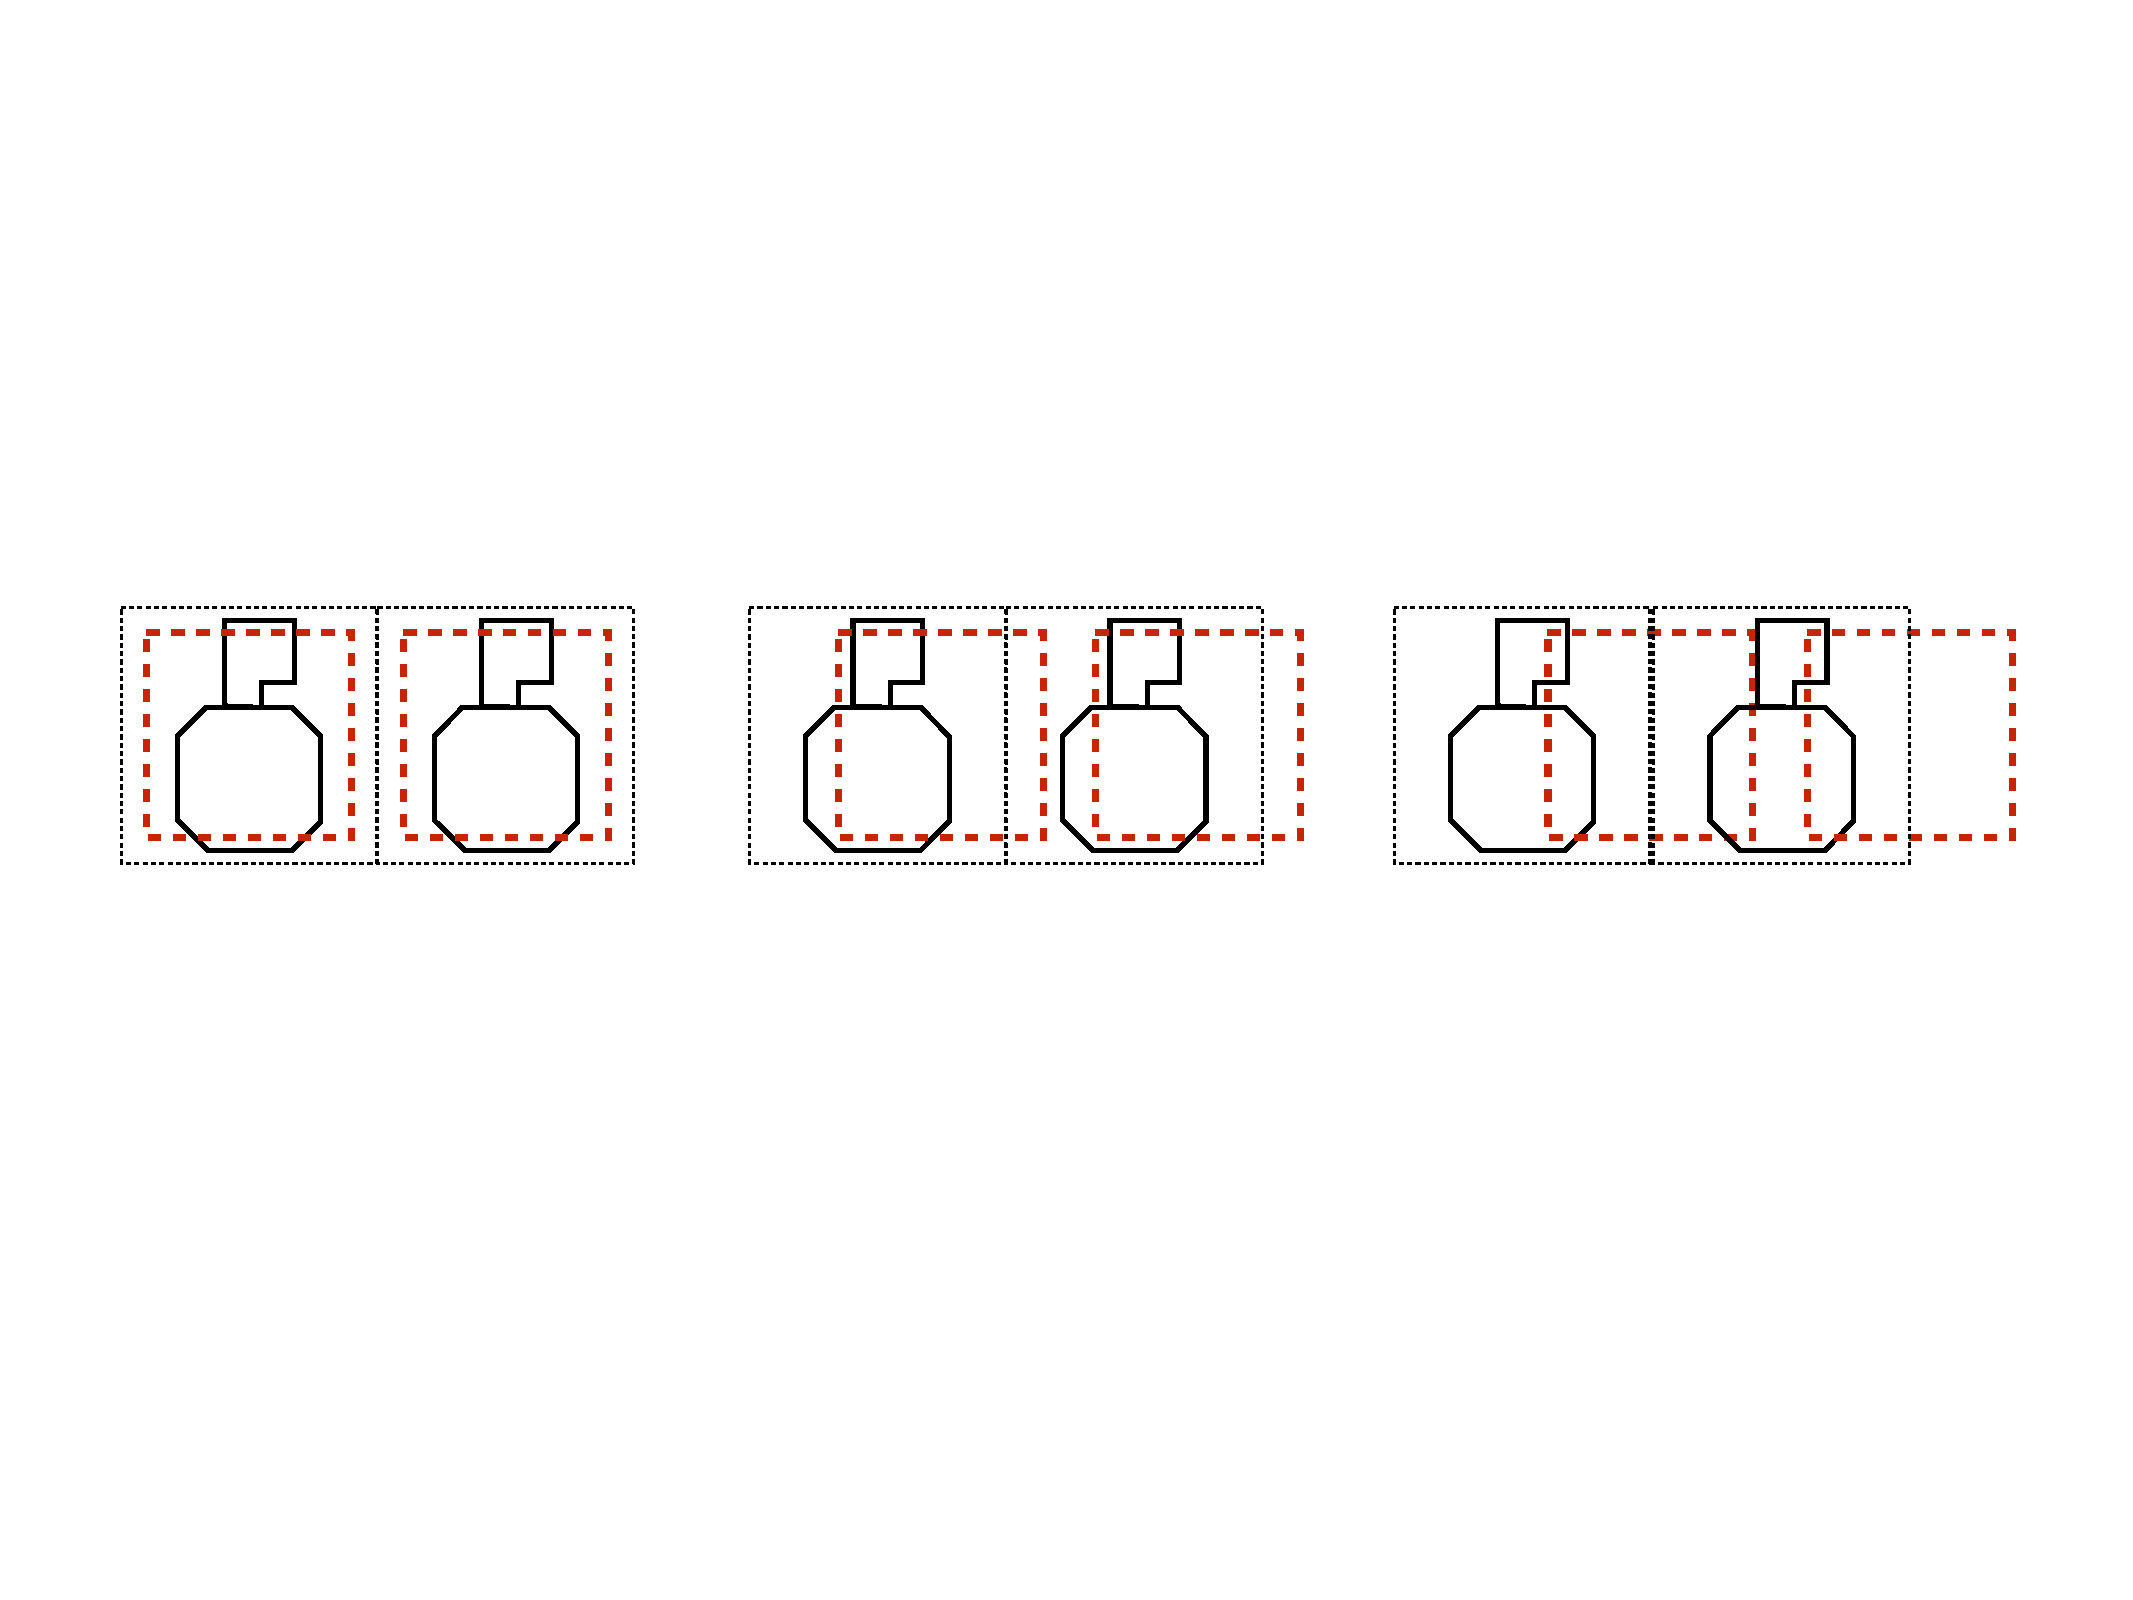
\includegraphics[width=1.0\textwidth]{CLICdpVertex/Plots/misalignedPads.pdf}
\caption[Schematic of alignment of CCPDv3 and CLICpix sensors studied in this analysis.]{Schematic of alignment of CCPDv3 and CLICpix sensors studied in this analysis.  The red dotted line represents the CCPDv3 and the solid black line represents the CLICpix.  From left to right; centred pixels, 1/4 offset (6.25 {\mu}m) and 1/2 offset (12.5 {\mu}m).}
\label{fig:alignment}
\end{figure}

\begin{table}[h!]
\centering
\begin{tabular}{ l l }
\hline
Assembly & Alignment \\ 
\hline
SET9 & Centred \\
SET10 & $\frac{1}{4}$ Offset \\
SET11 & $\frac{1}{2}$ Offset \\
SET12 & Centred \\
SET13 & Centred \\
SET14 & $\frac{1}{2}$ Offset \\
SET15 & Centred \\
SET16 & $\frac{1}{2}$ Offset \\
\hline
\end{tabular}
\caption[Description of alignment of sensors.]{Description of alignment of sensors.}
\label{table:alignment}
\end{table}

The pitch of the pixels produced was 25 {\mu}m and the matrix size was 64$\times$64.  The full details of the gluing process can be found here (CERN NOTE CITE) along with a study into the absolute precision of the manufacturing procedure.  It was found that for devices constructed in an identical fashion to those considered here, the glue layer thicknesses were less than 1 {\mu}m and the precision on the pixel positioning was less than 0.5 {\mu}m.  

\section{Device Characterisation}

This section describes the electrical tests that were performed on the sensor designed to determine the properties of the HV-CMOS and CLICpix.  

\subsection{CLICPix Calibration}

\subsubsection{Experimental Setup}
A radioactive source, $\text{Sr}^{90}$, calibration that was applied to the sensors is presented here.  In this procedure the unstable $\text{Sr}^{90}$ undergoes $\beta^{-}$ decay to form $\text{Y}^{90}$.  The $\text{Y}^{90}$, as it too is unstable, undergoes $\beta^{-}$ decay to form $\text{Z}^{90}$, which is stable.  Each $\beta^{-}$ decays produce an $\text{e}^{-}$ and a $\bar{\nu_{e}}$, and it is the $\text{e}^{-}$ that are used to test the sensitivity of the sensor.  The $\text{Sr}^{90}$ source used had an activity of 29.6 MBq.  

This radioactive source was positioned directly on top of the sensors and measurements were made of both the ToT output from the CLICpix and the HV-CMOS analogue signal for individual pixels on the sensor.  The on-pixel event counter was used to veto all events where multiple hits occurred within the time window for a given event.  

\begin{figure}
\centering
\subfloat[]{\label{fig:pulseshape1}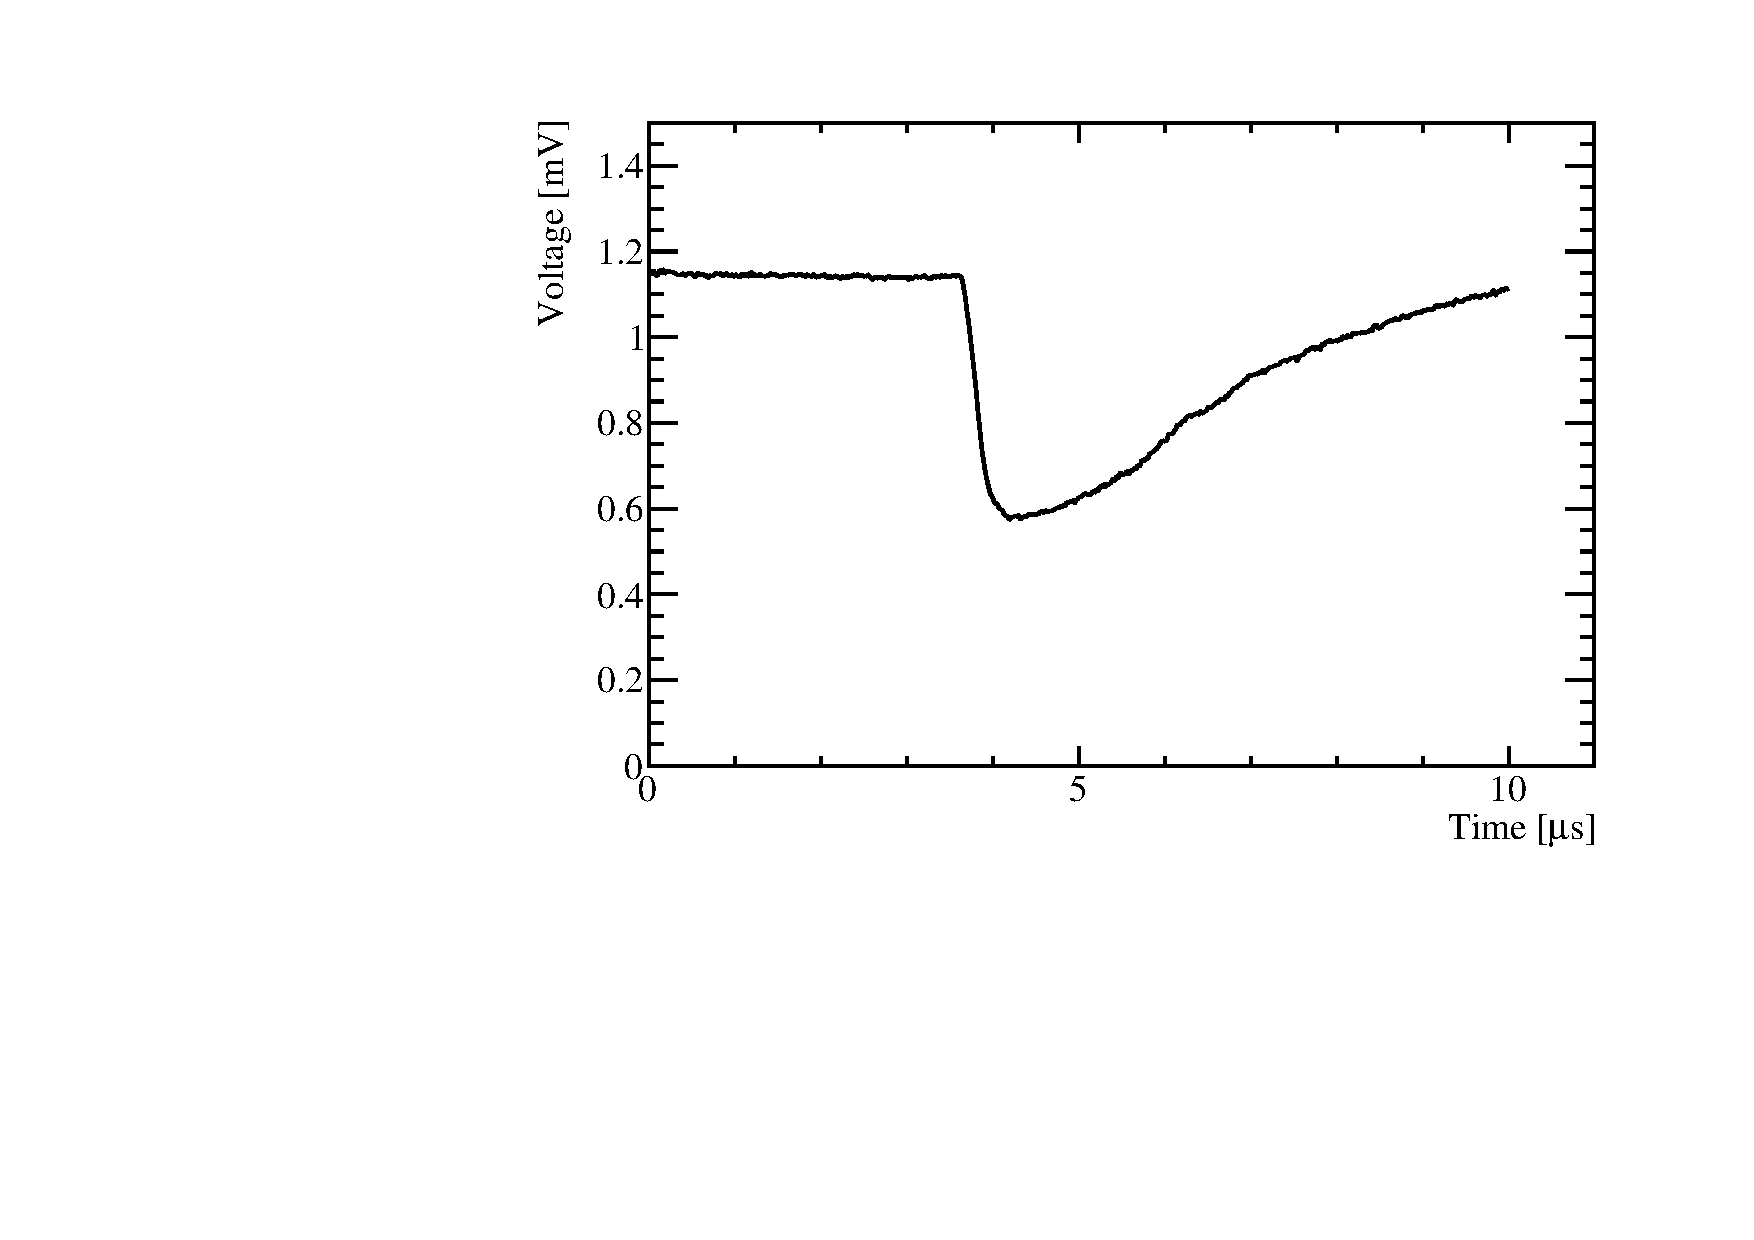
\includegraphics[width=0.5\textwidth]{CLICdpVertex/Plots/HV-CMOS/Frames/PulseShape01000NoOffset.pdf}}
\subfloat[]{\label{fig:pulseshape2}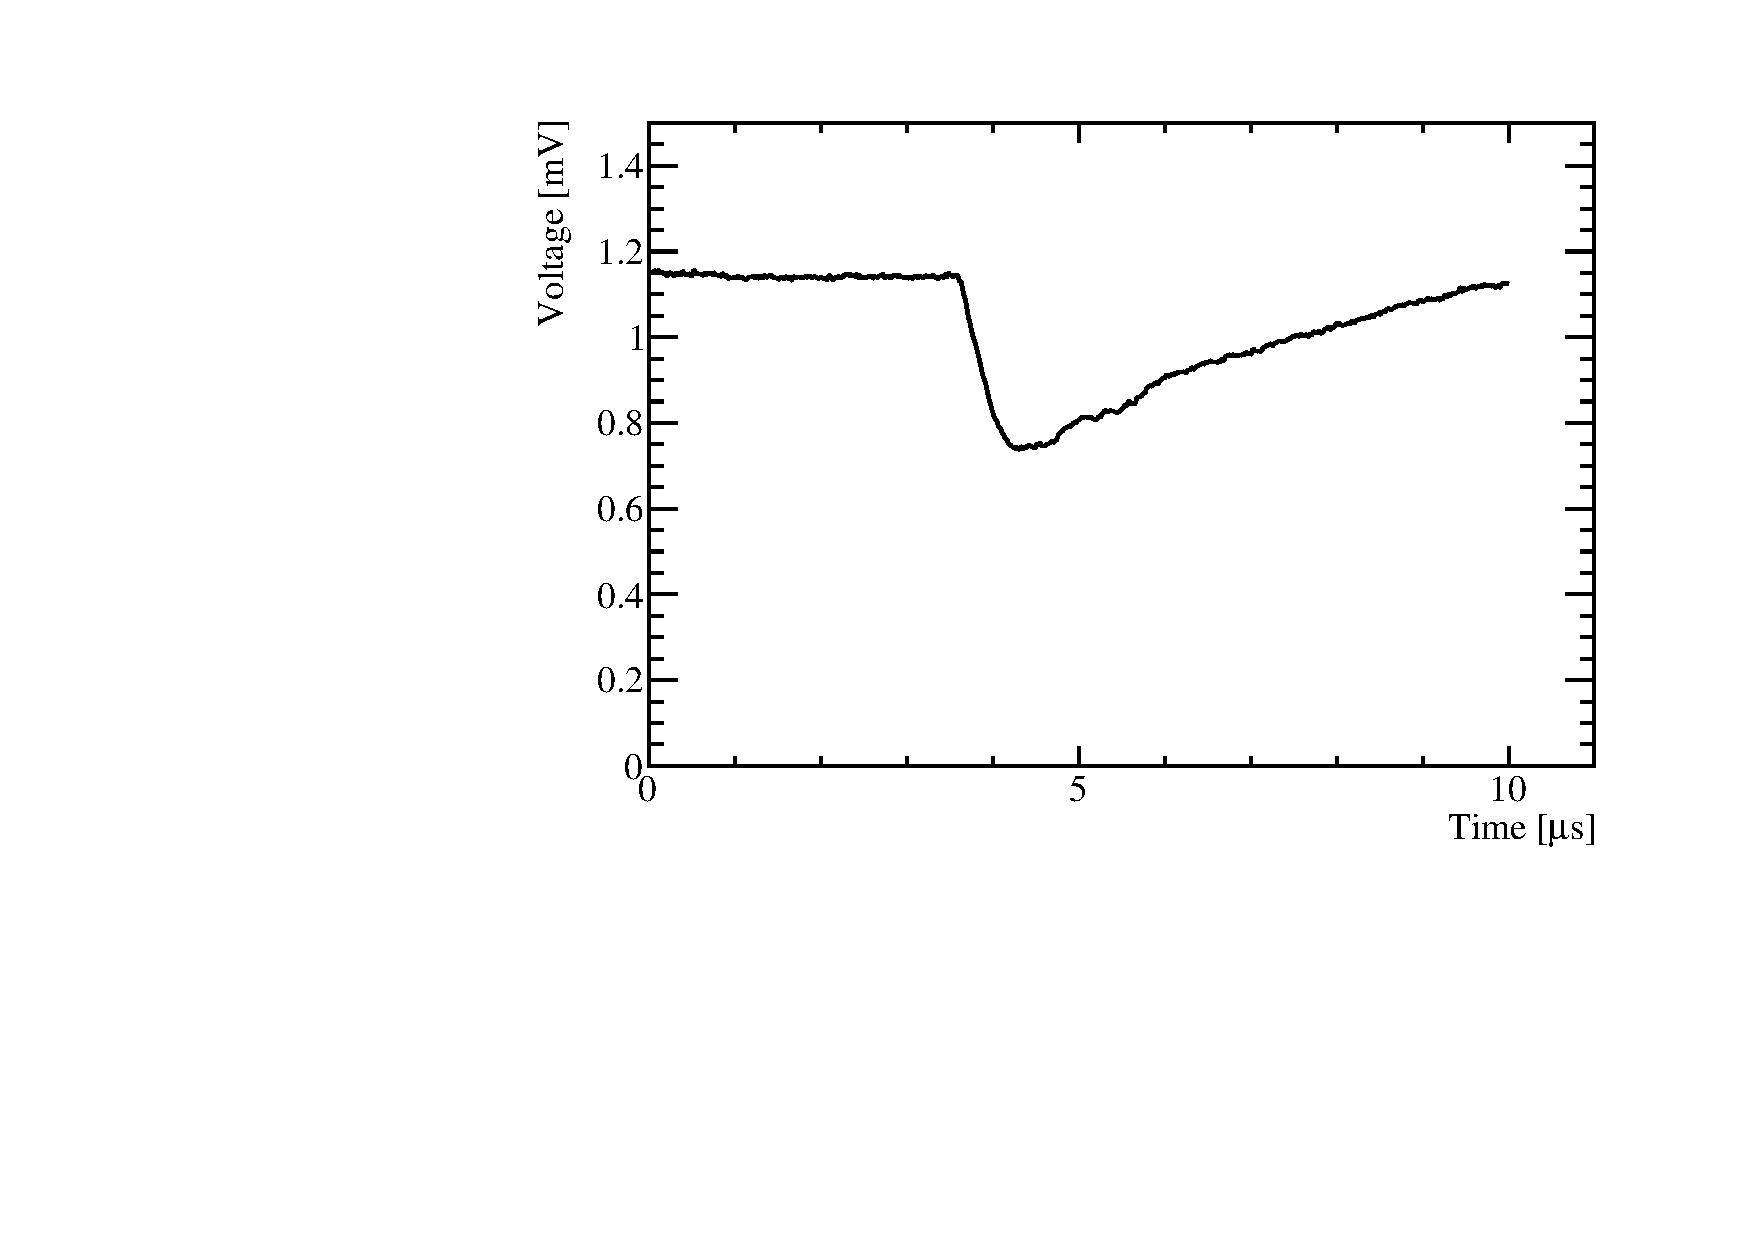
\includegraphics[width=0.5\textwidth]{CLICdpVertex/Plots/HV-CMOS/Frames/PulseShape01005NoOffset.pdf}}\hfill
\subfloat[]{\label{fig:pulseshape3}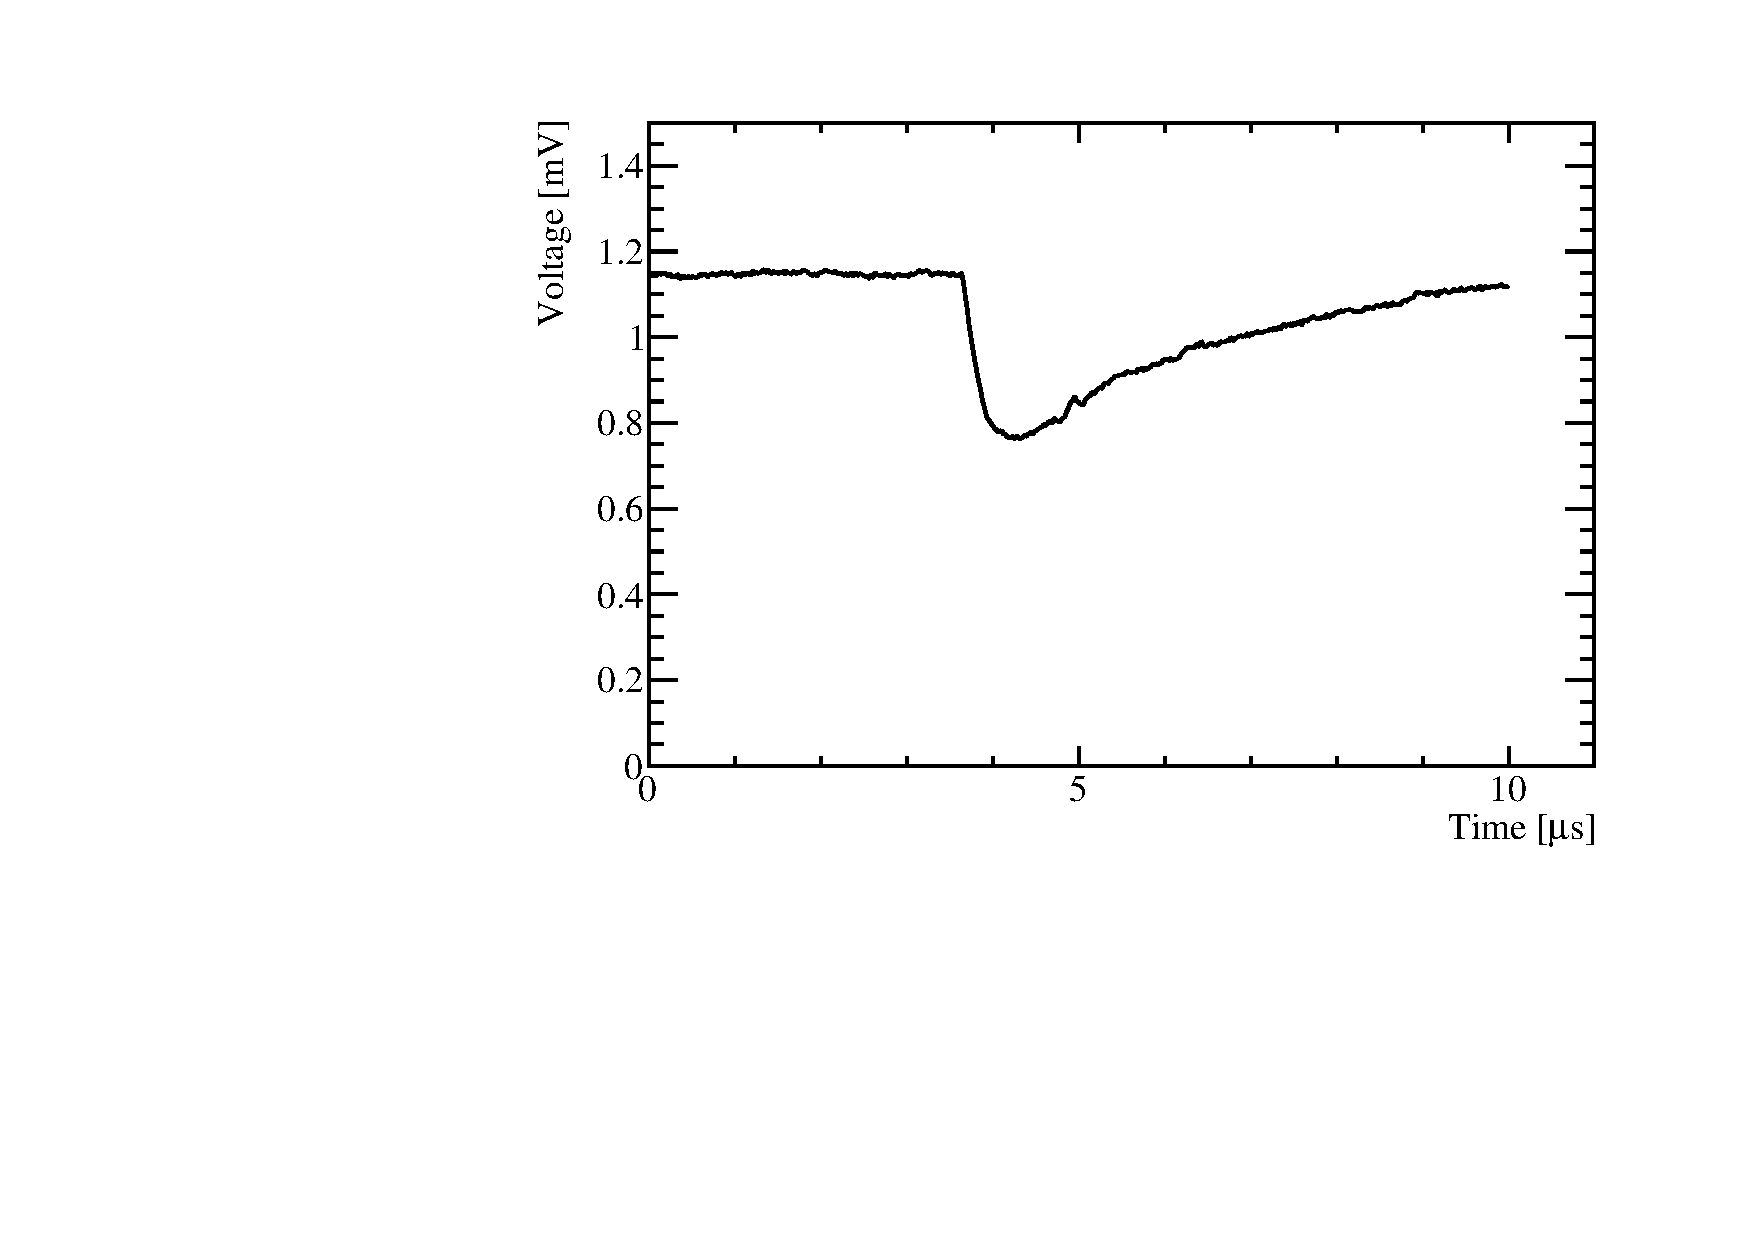
\includegraphics[width=0.5\textwidth]{CLICdpVertex/Plots/HV-CMOS/Frames/PulseShape01006NoOffset.pdf}}
\subfloat[]{\label{fig:pulseshape4}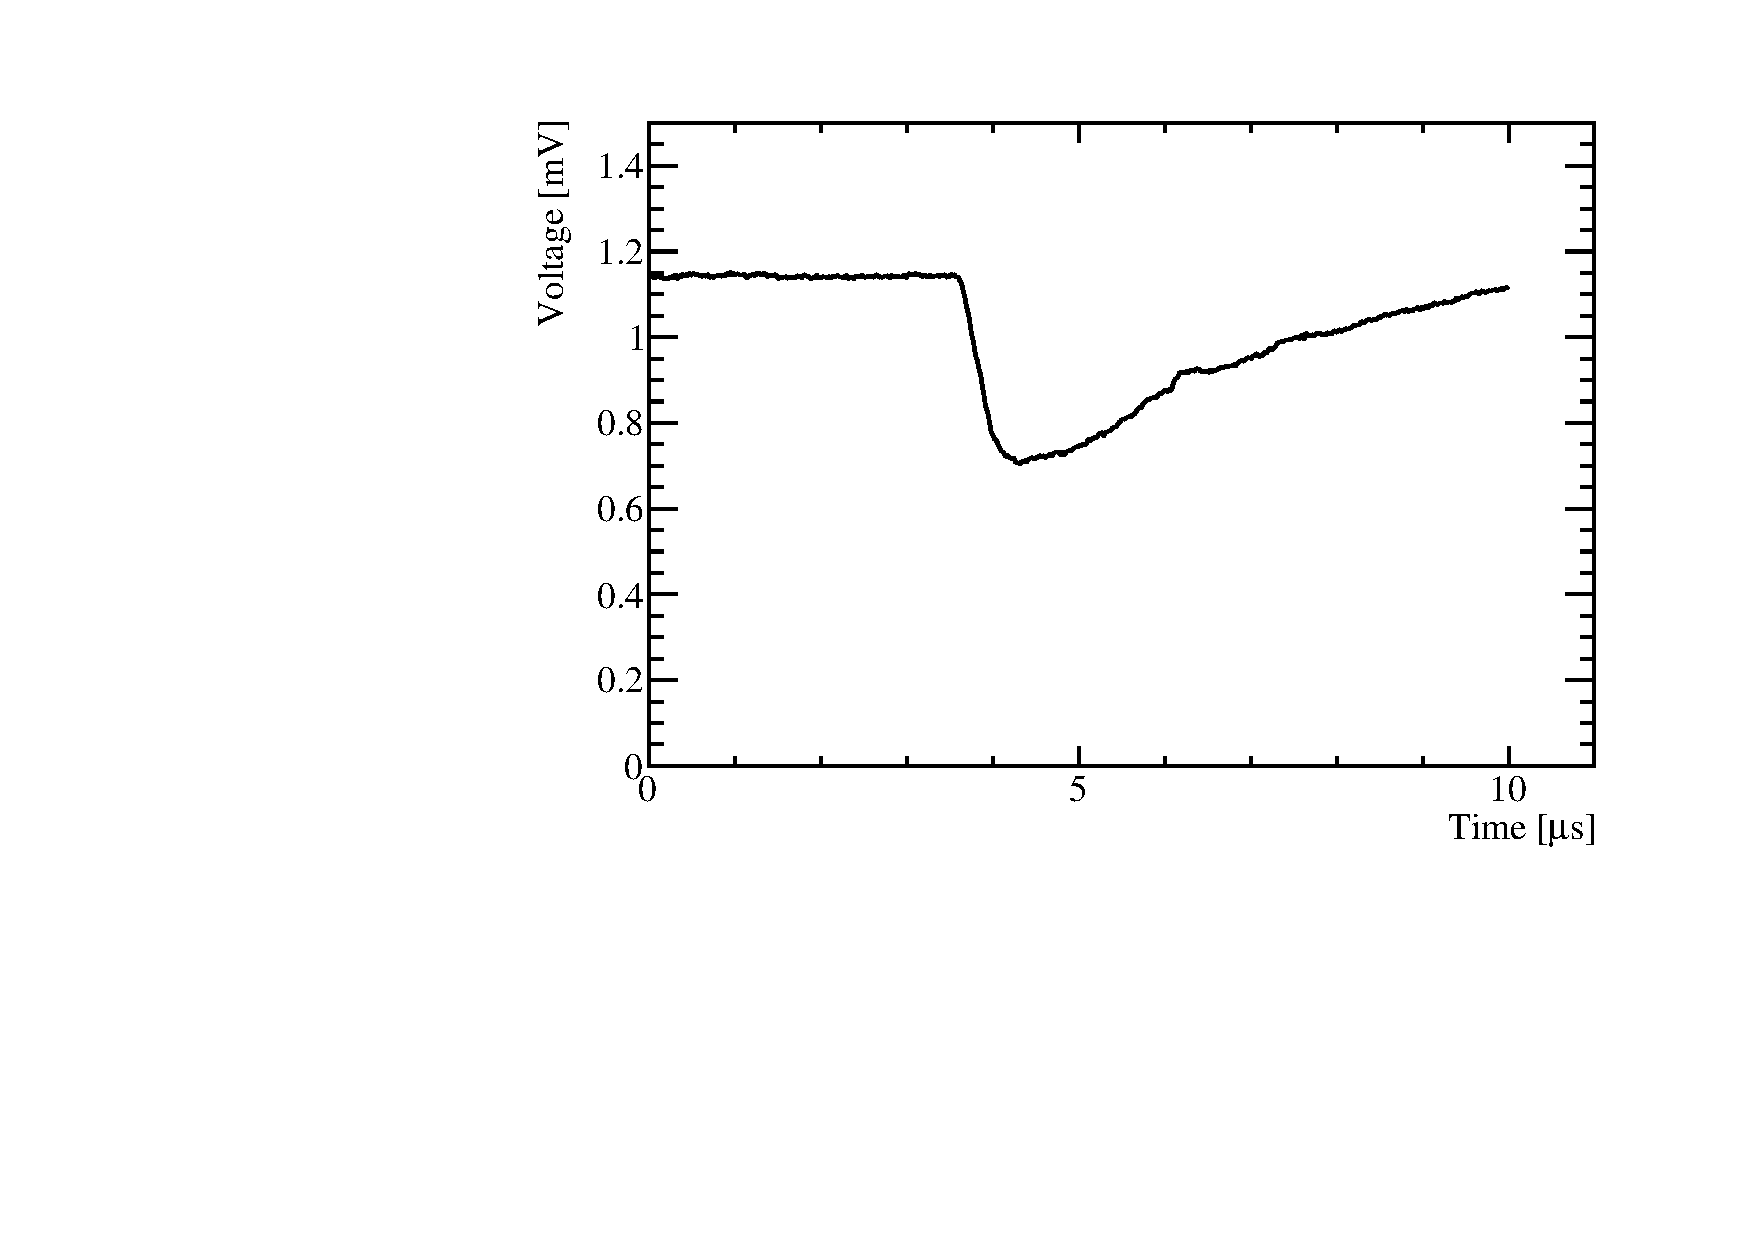
\includegraphics[width=0.5\textwidth]{CLICdpVertex/Plots/HV-CMOS/Frames/PulseShape01008NoOffset.pdf}}
\caption[HV-CMOS voltage as a function of time for pulses created by radioactive strontium 90 source.]{HV-CMOS voltage as a function of time for pulses created by radioactive $\text{Sr}^{90}$ source.}
\label{fig:pulseshapes}
\end{figure}

The HV-CMOS analogue output has a DC output of $\approx 1.15$ V and saturation occurs around a signal height of 700 mV.  Examples of the HV-CMOS output can be found in figure \ref{fig:pulseshapes}.

\subsubsection{Analysis}
The quantities of interest related to the HV-CMOS output are the pulse height and a rise time.  The offset voltage was subtracted from the HV-CMOS analogue output and the pulse height inverted before the following analysis was applied.

\begin{figure}
\centering
\subfloat[\textbf{Rise time.}  The arrows show the change in time and voltage as the pulse goes from 10\% to 90\% of the raw pulse height.  This time is used as the definition of the rise time in the subsequent analysis.]{\label{fig:pulseshapeanalysistime}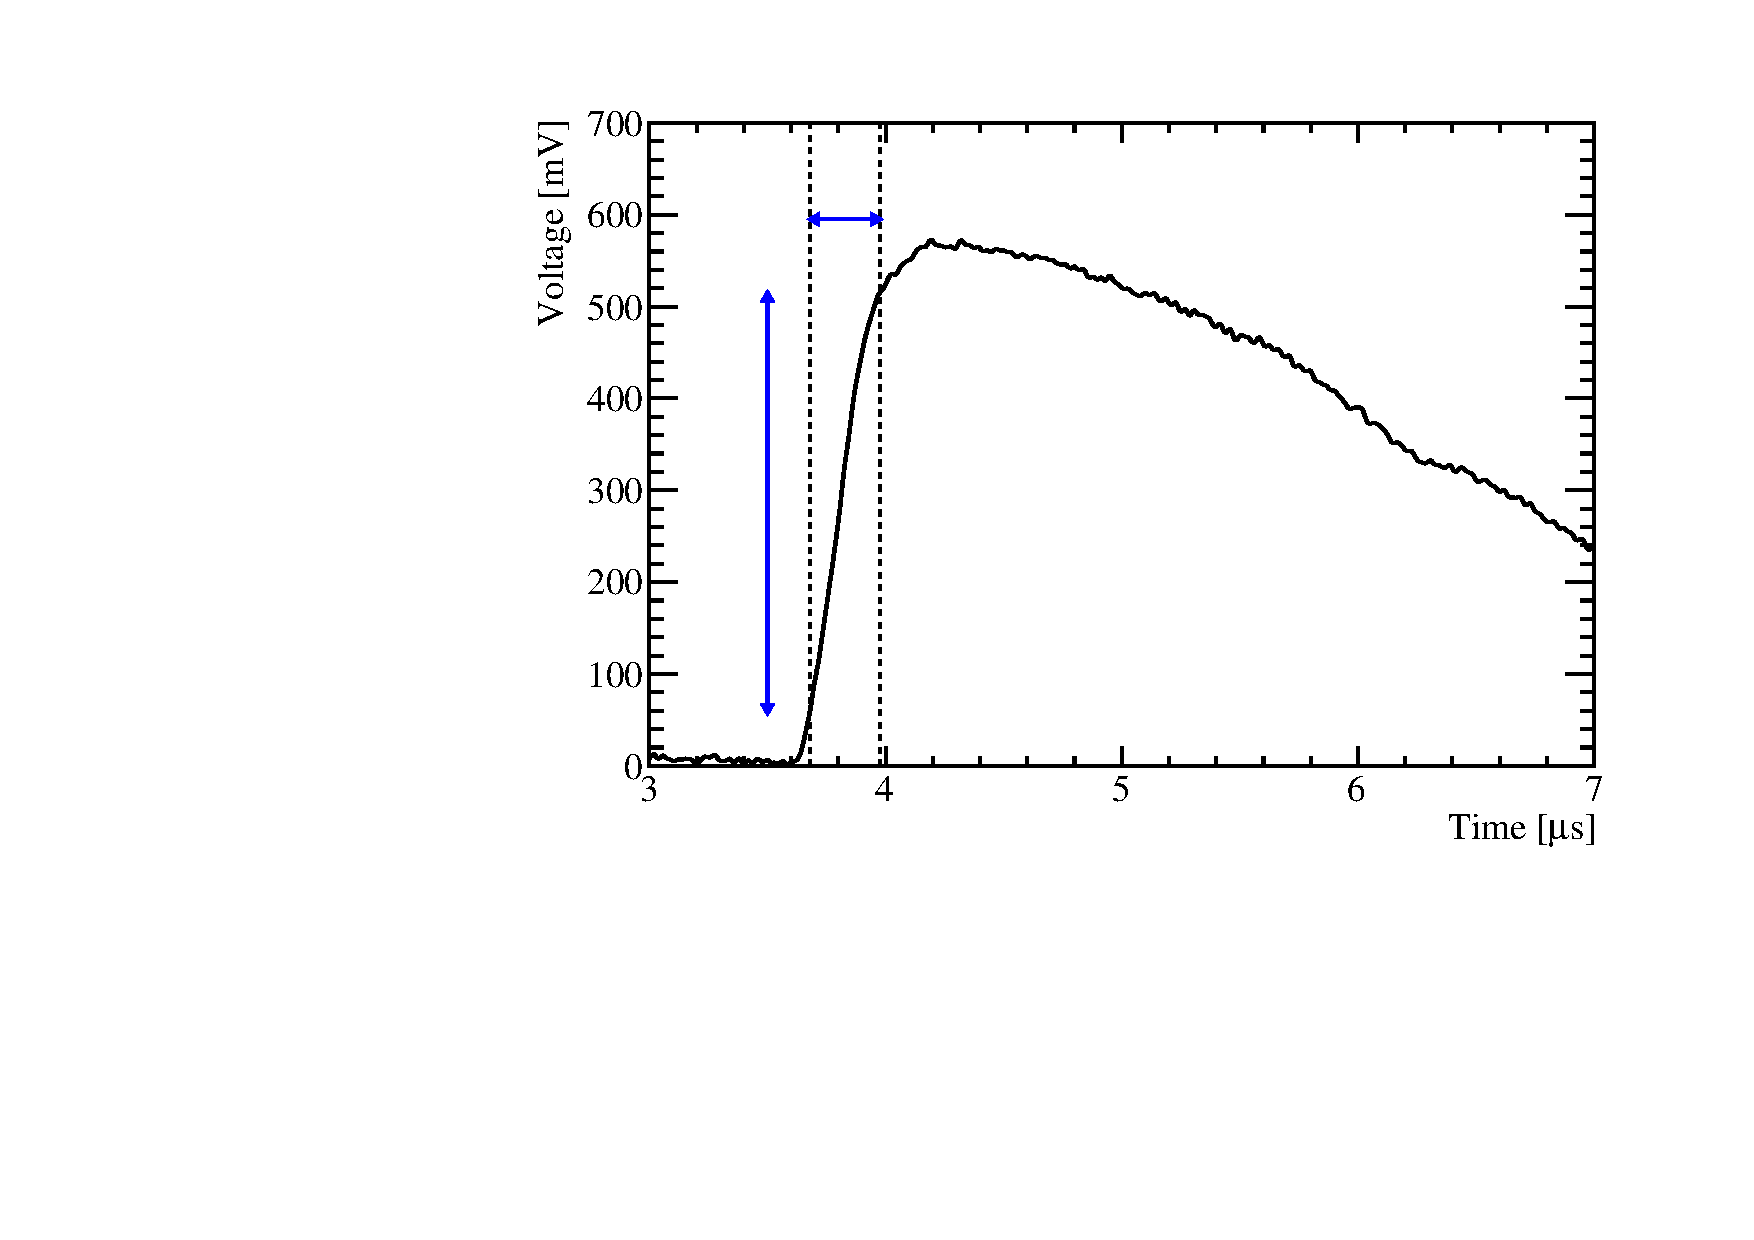
\includegraphics[width=0.5\textwidth]{CLICdpVertex/Plots/HV-CMOS/Frames/PulseShape01000FittingRiseTime.pdf}}
\subfloat[\textbf{Pulse height.} The red dotted line is a Gaussian fit to the peak of the pulse.  The peak is defined as data points where the voltage is in excess of 90\% of the raw pulse height.]{\label{fig:pulseshapeanalysisvoltage}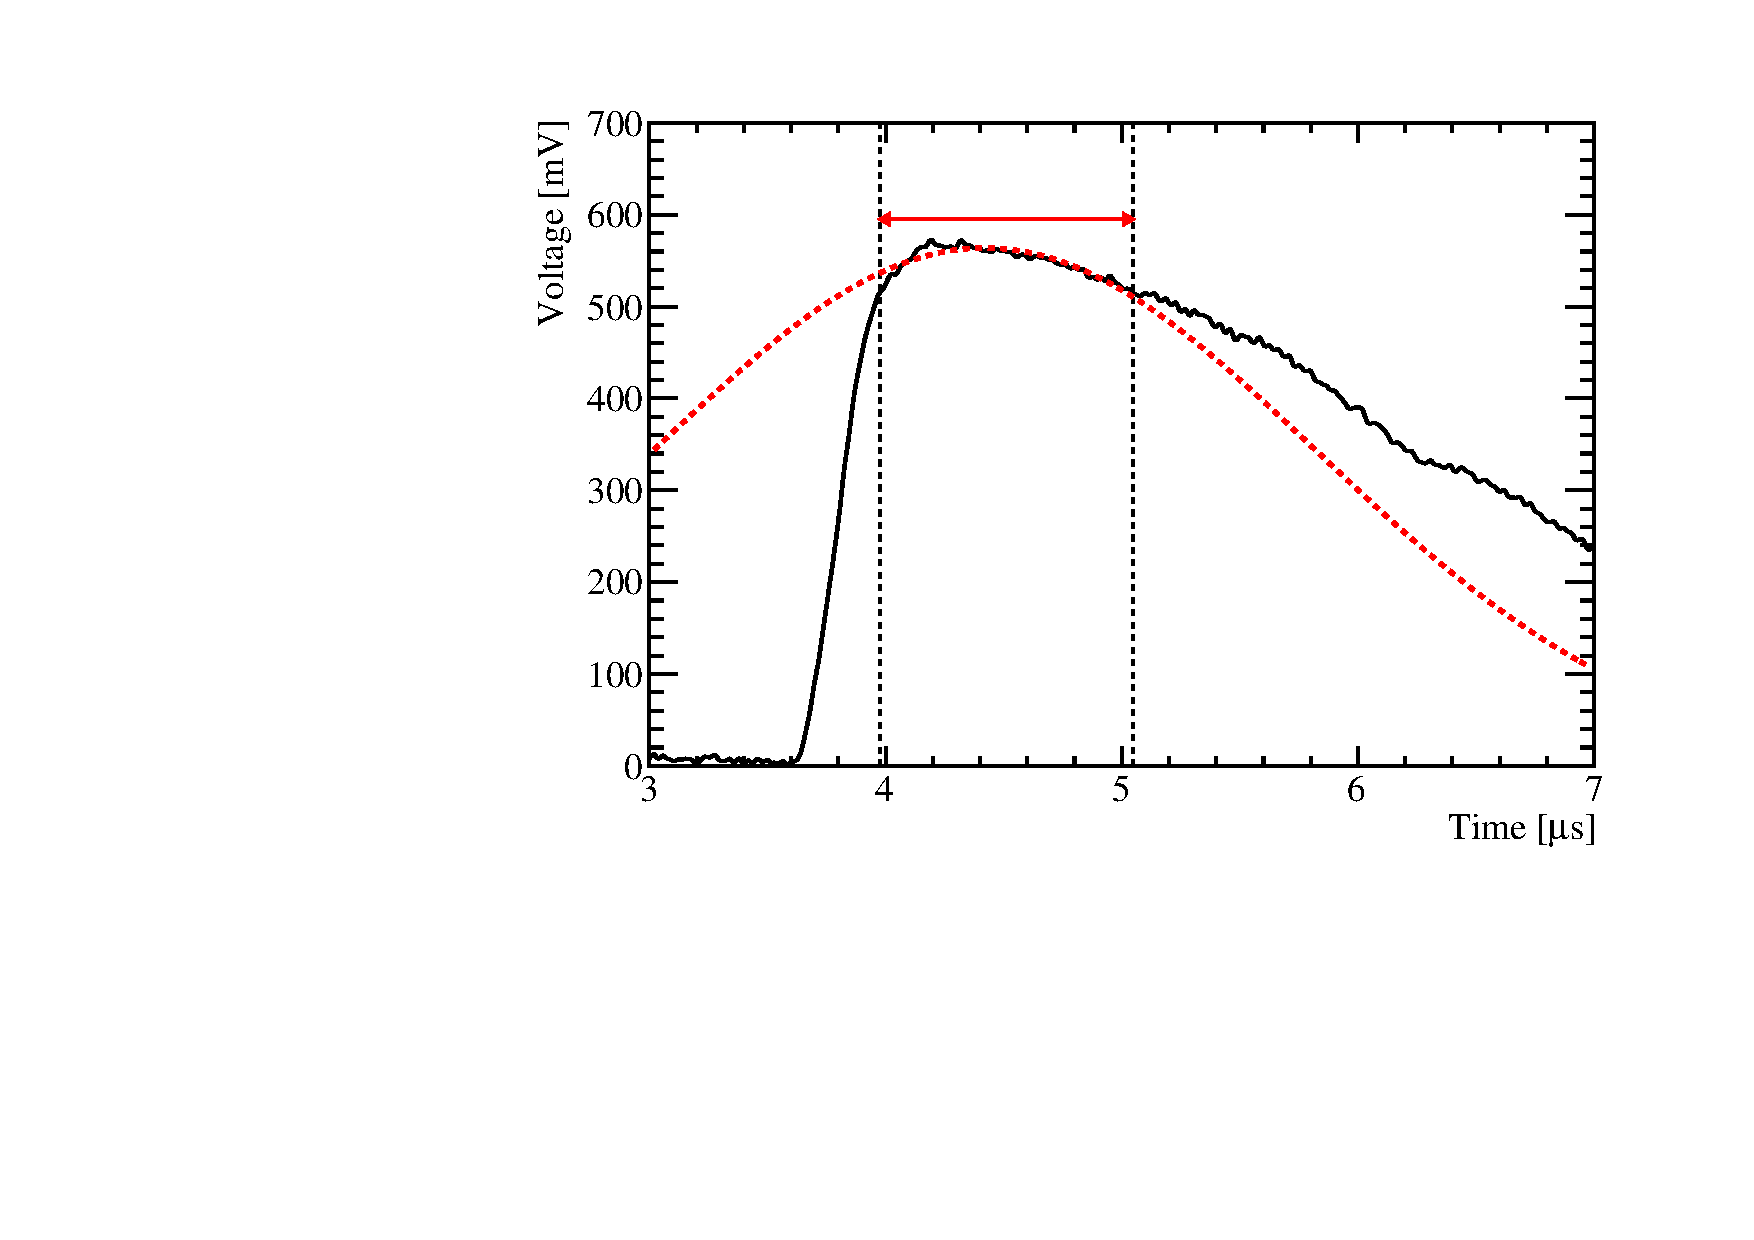
\includegraphics[width=0.5\textwidth]{CLICdpVertex/Plots/HV-CMOS/Frames/PulseShape01000FittingVoltage.pdf}}\hfill
\caption[Analysis of HV-CMOS voltage as a function of time for pulses created by radioactive strontium 90 source.]{Analysis of HV-CMOS voltage as a function of time for pulses created by radioactive $\text{Sr}^{90}$ source.}
\label{fig:pulseshapeanalysis}
\end{figure}

The pulse height was taken as the mean of a Gaussian fit to the peak of the HV-CMOS output voltage distribution.  Such peaks were defined as the data points set that were at or above 90\% of the raw peak height, the maximum voltage change recorded.  The application of a Gaussian fit provides a more robust metric for categorising the pulse height that is not dependant on minor fluctuations in the voltage.  The rise time was calculated as the time taken for the voltage to go from 10\% to 90\% of the raw peak height.  This definition also makes the rise time metric more robust against fluctuations changing the absolute peak height.  Examples of the calculation of these metrics for a given pulse are shown in figure \ref{fig:pulseshapeanalysis}.

For each device the HV-CMOS pulse output was recorded for 15 pixels running along one edge of the 64 $\times$ 64 matrix.  In the subsequent section the mean ToT and pulse height are plotted by first binning the distribution, from all pixels considered, of either ToT or rise time against pulse height using bins of 0.25 mV.  Then the mean of the variable of interest is plotted for each bin.  The error bars shown in the following section correspond to the standard deviation of the bin contents for each bin.   

\subsubsection{Results}


\begin{figure}
\centering
\subfloat[Mean rise time for all samples.]{\label{fig:risetime1}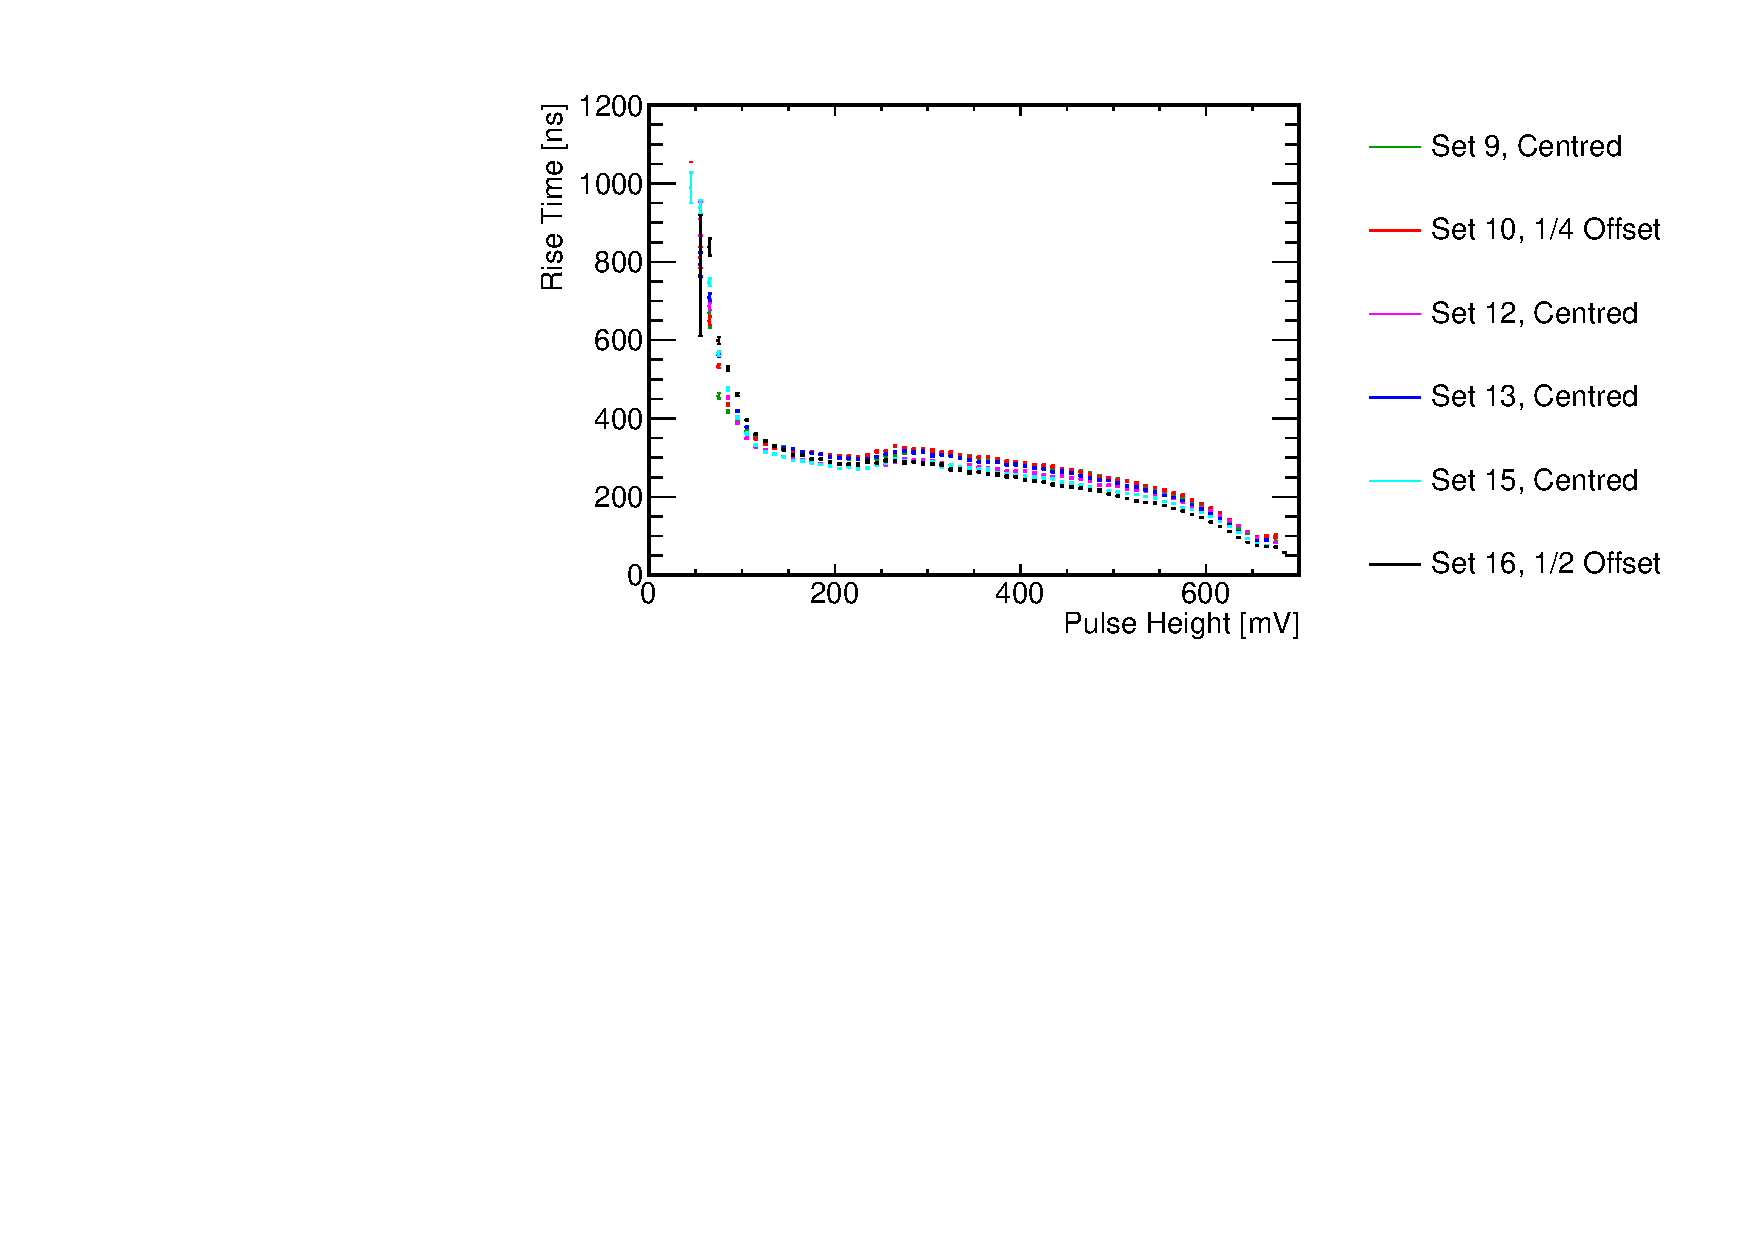
\includegraphics[width=1.0\textwidth]{CLICdpVertex/Plots/RadSourceAnalysis/AllSETs_RiseTime_PulseHeight.pdf}}\hfill
\subfloat[Mean rise time with error bars corresponding to standard deviation of binned rise time distribution for selected sample.]{\label{fig:risetime2}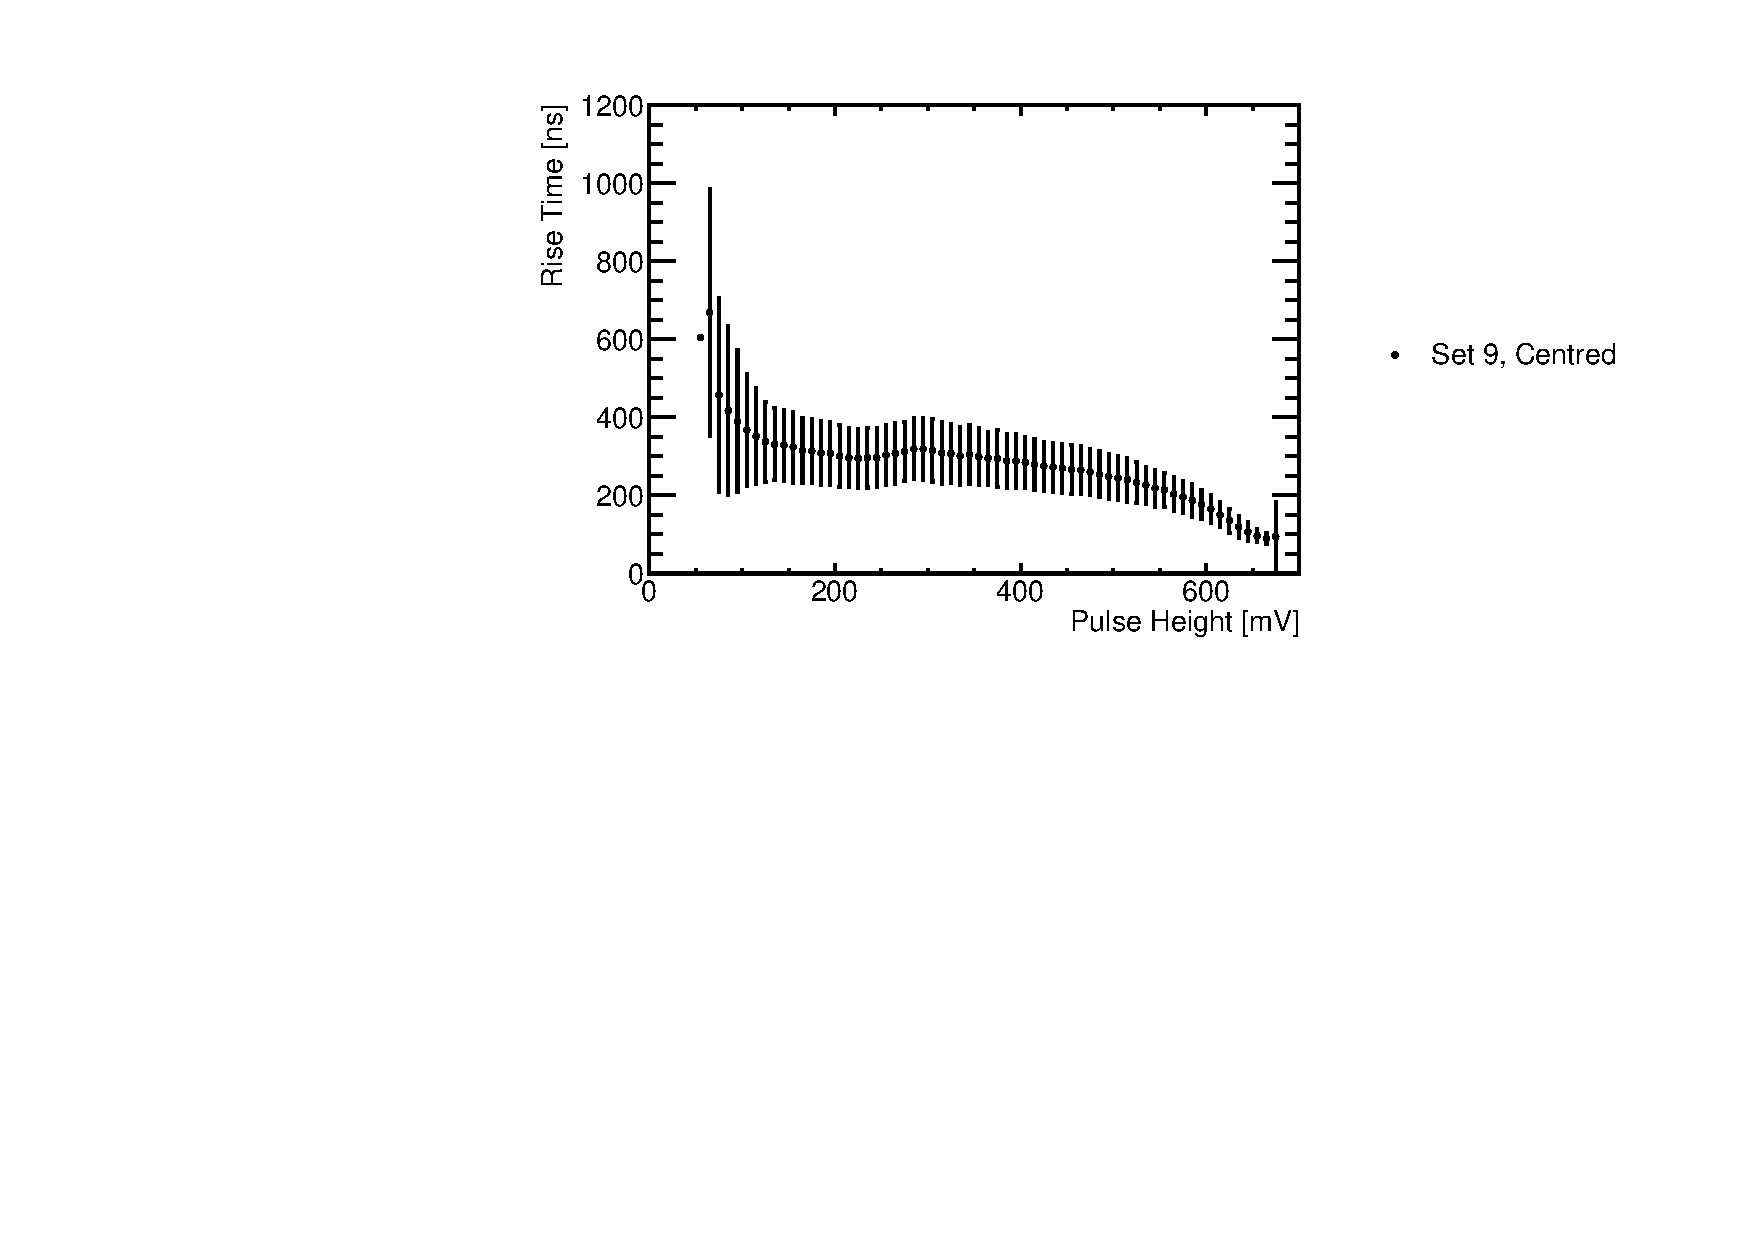
\includegraphics[width=1.0\textwidth]{CLICdpVertex/Plots/RadSourceAnalysis/AllSETs_RiseTime_PulseHeight_Width.pdf}}
\caption[HV-CMOS voltage rise time as a function of pulse height.]{HV-CMOS voltage rise time as a function of pulse height.}
\label{fig:risetime}
\end{figure}

\begin{figure}
\centering
\subfloat[Mean ToT for all samples.]{\label{fig:tot1}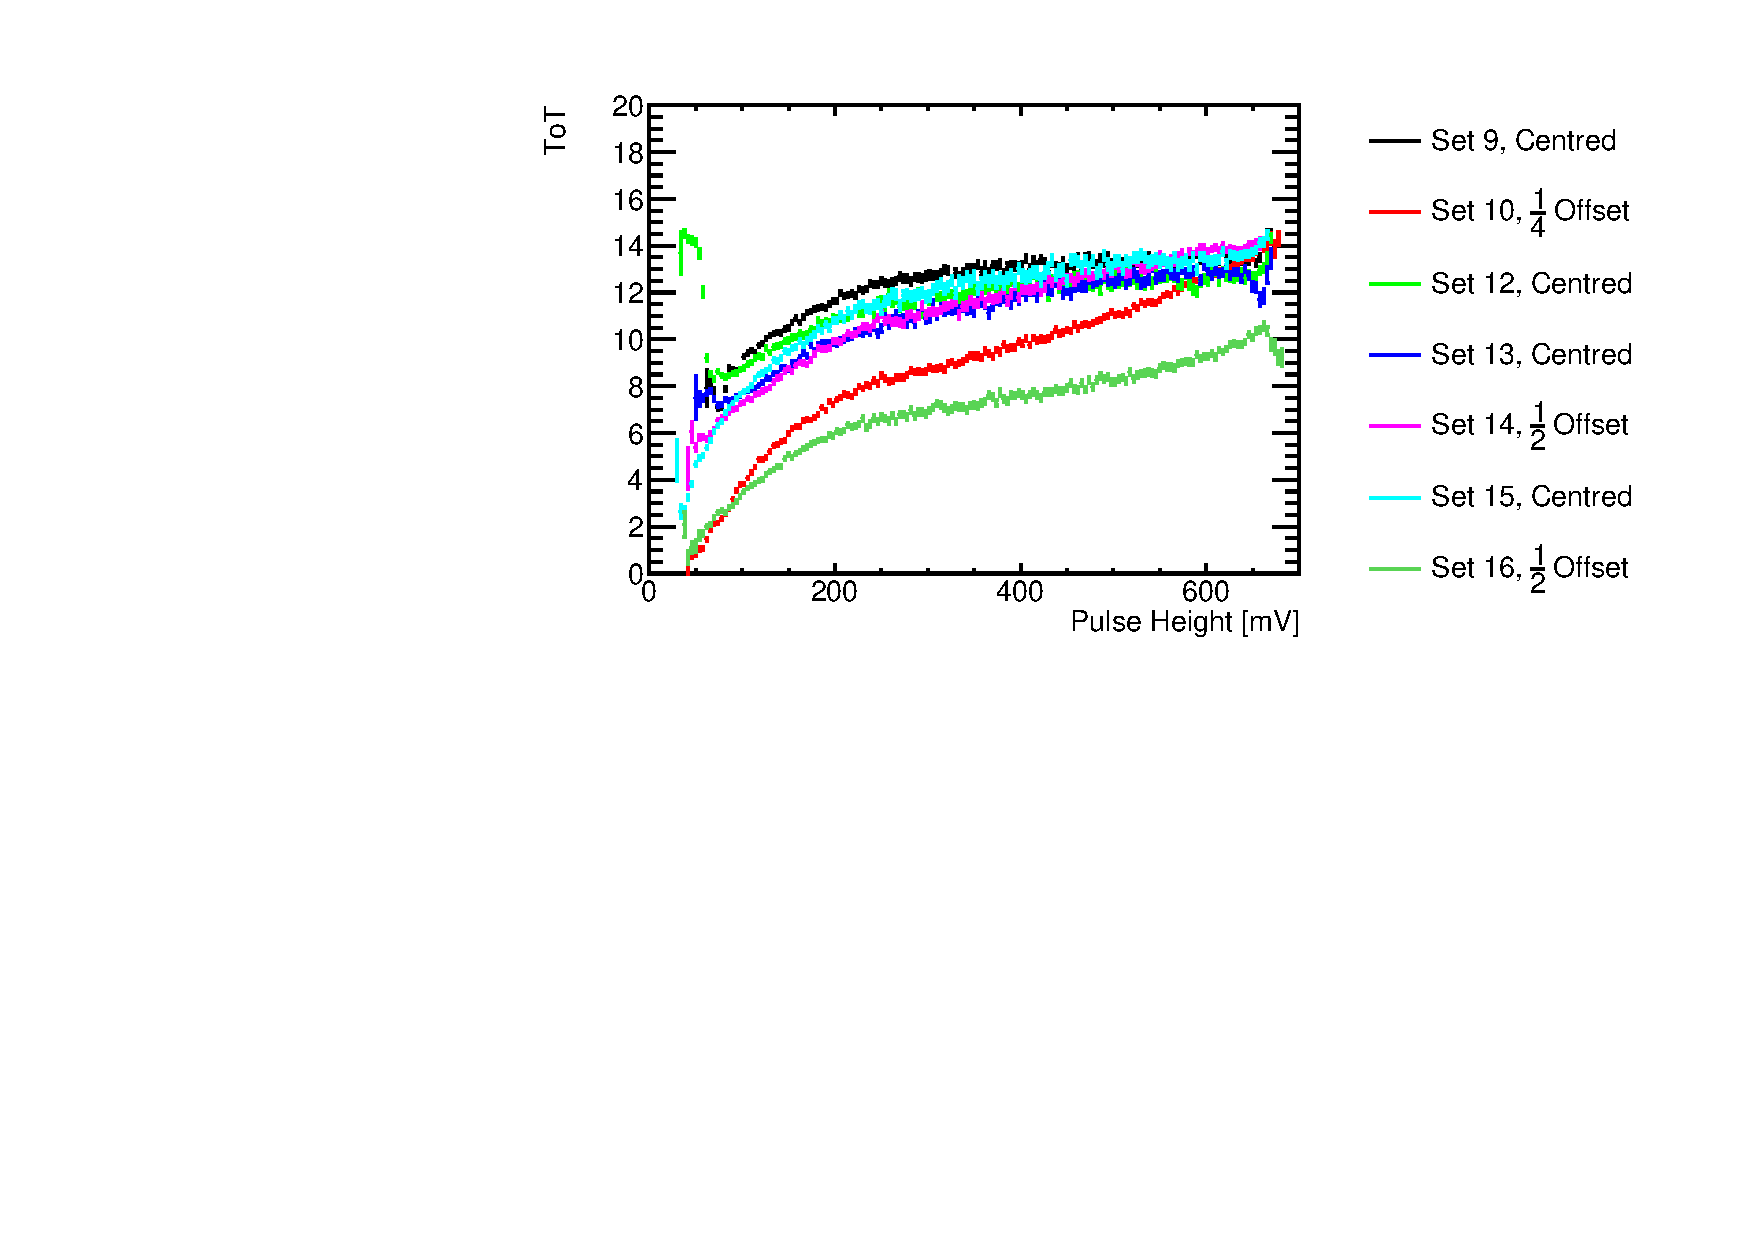
\includegraphics[width=1.0\textwidth]{CLICdpVertex/Plots/RadSourceAnalysis/AllSETs_TargetTot_PulseHeight.pdf}}\hfill
\subfloat[Mean ToT with error bars corresponding to standard deviation of binned ToT distribution for selected sample.]{\label{fig:tot2}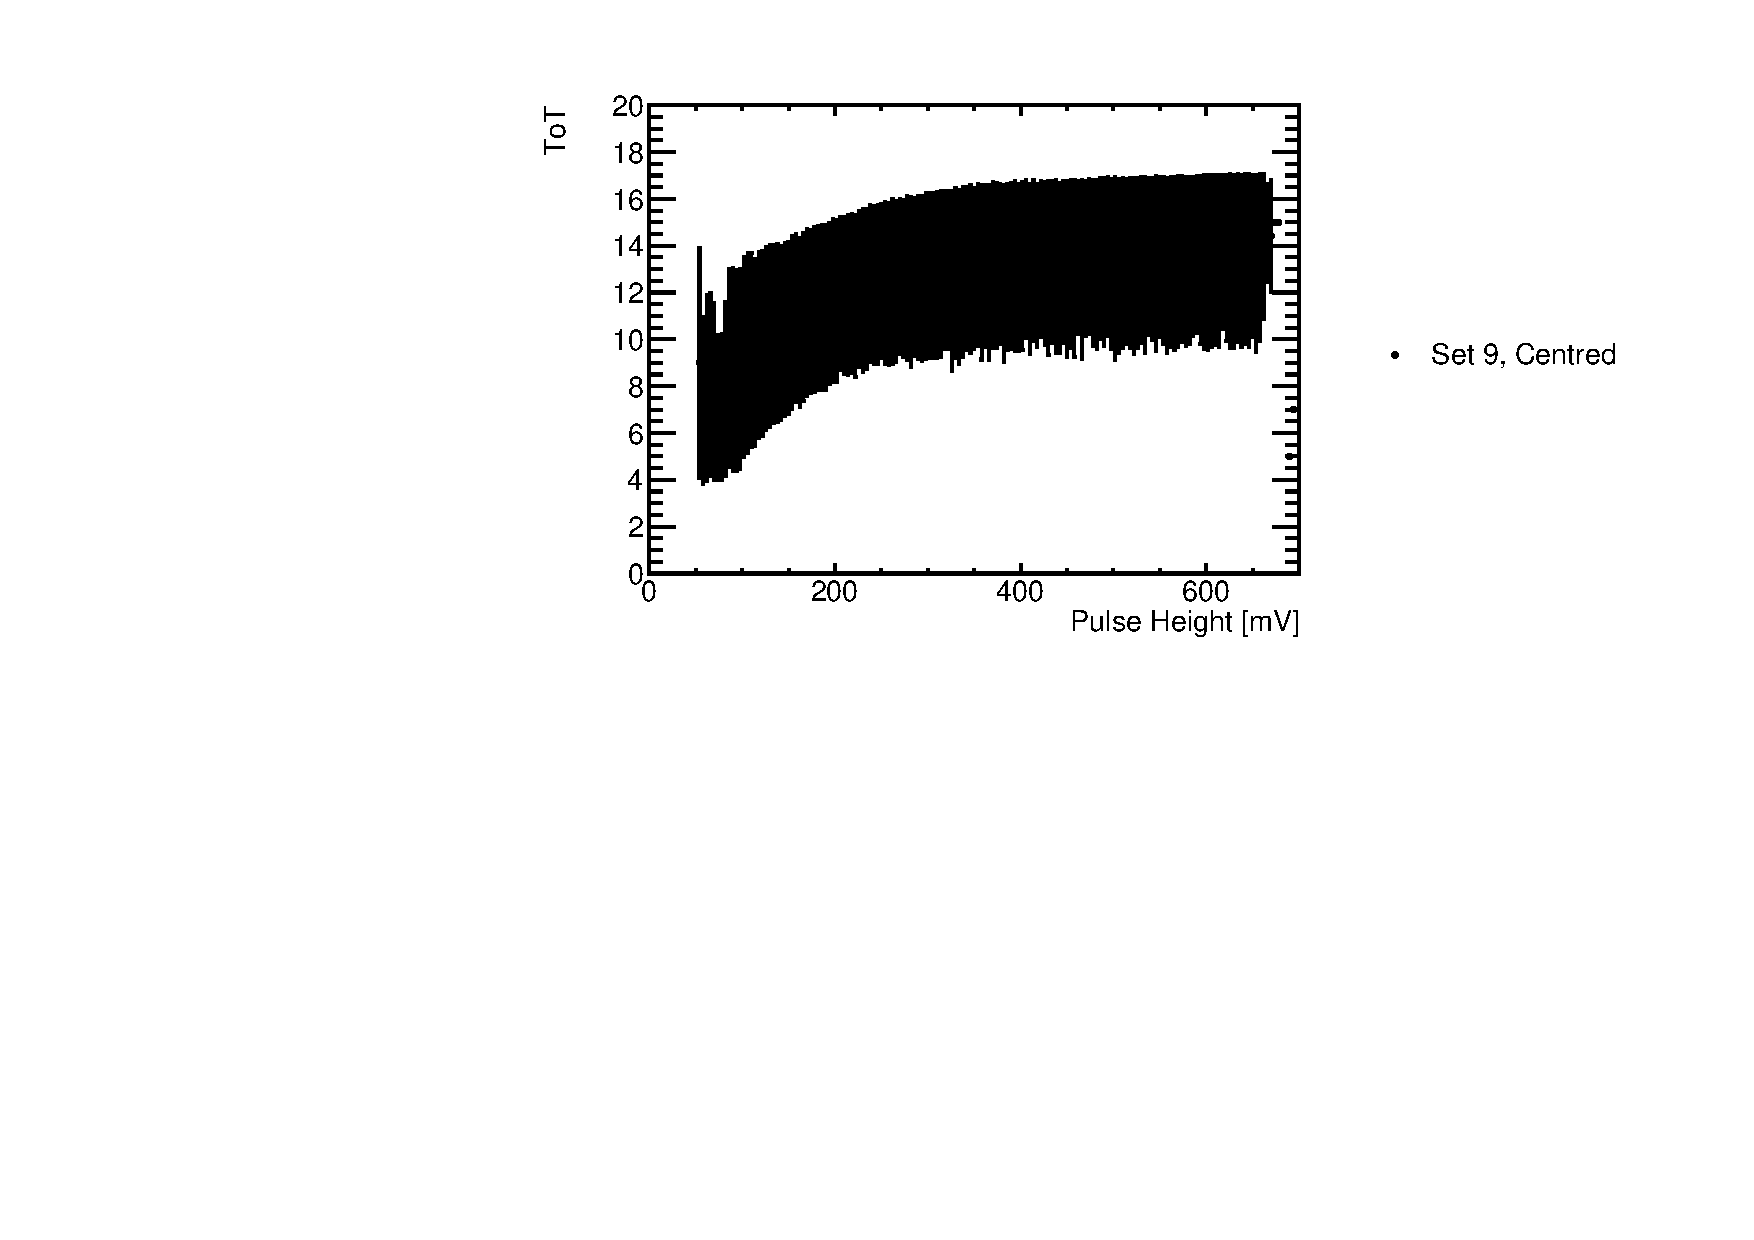
\includegraphics[width=1.0\textwidth]{CLICdpVertex/Plots/RadSourceAnalysis/AllSETs_TargetTot_PulseHeight_Width.pdf}}
\caption[CLICpix ToT as a function of HV-CMOS voltage pulse height.]{CLICpix ToT as a function of HV-CMOS voltage pulse height.}
\label{fig:tot}
\end{figure}











\subsection{Cross Couplings}
ToT on adjacent cells vs pulse heights.  No charge sharing apparent except for SET16.  Possible issues with manufacturing other offset samples as some charge sharing is expcted.

\begin{figure}
\centering
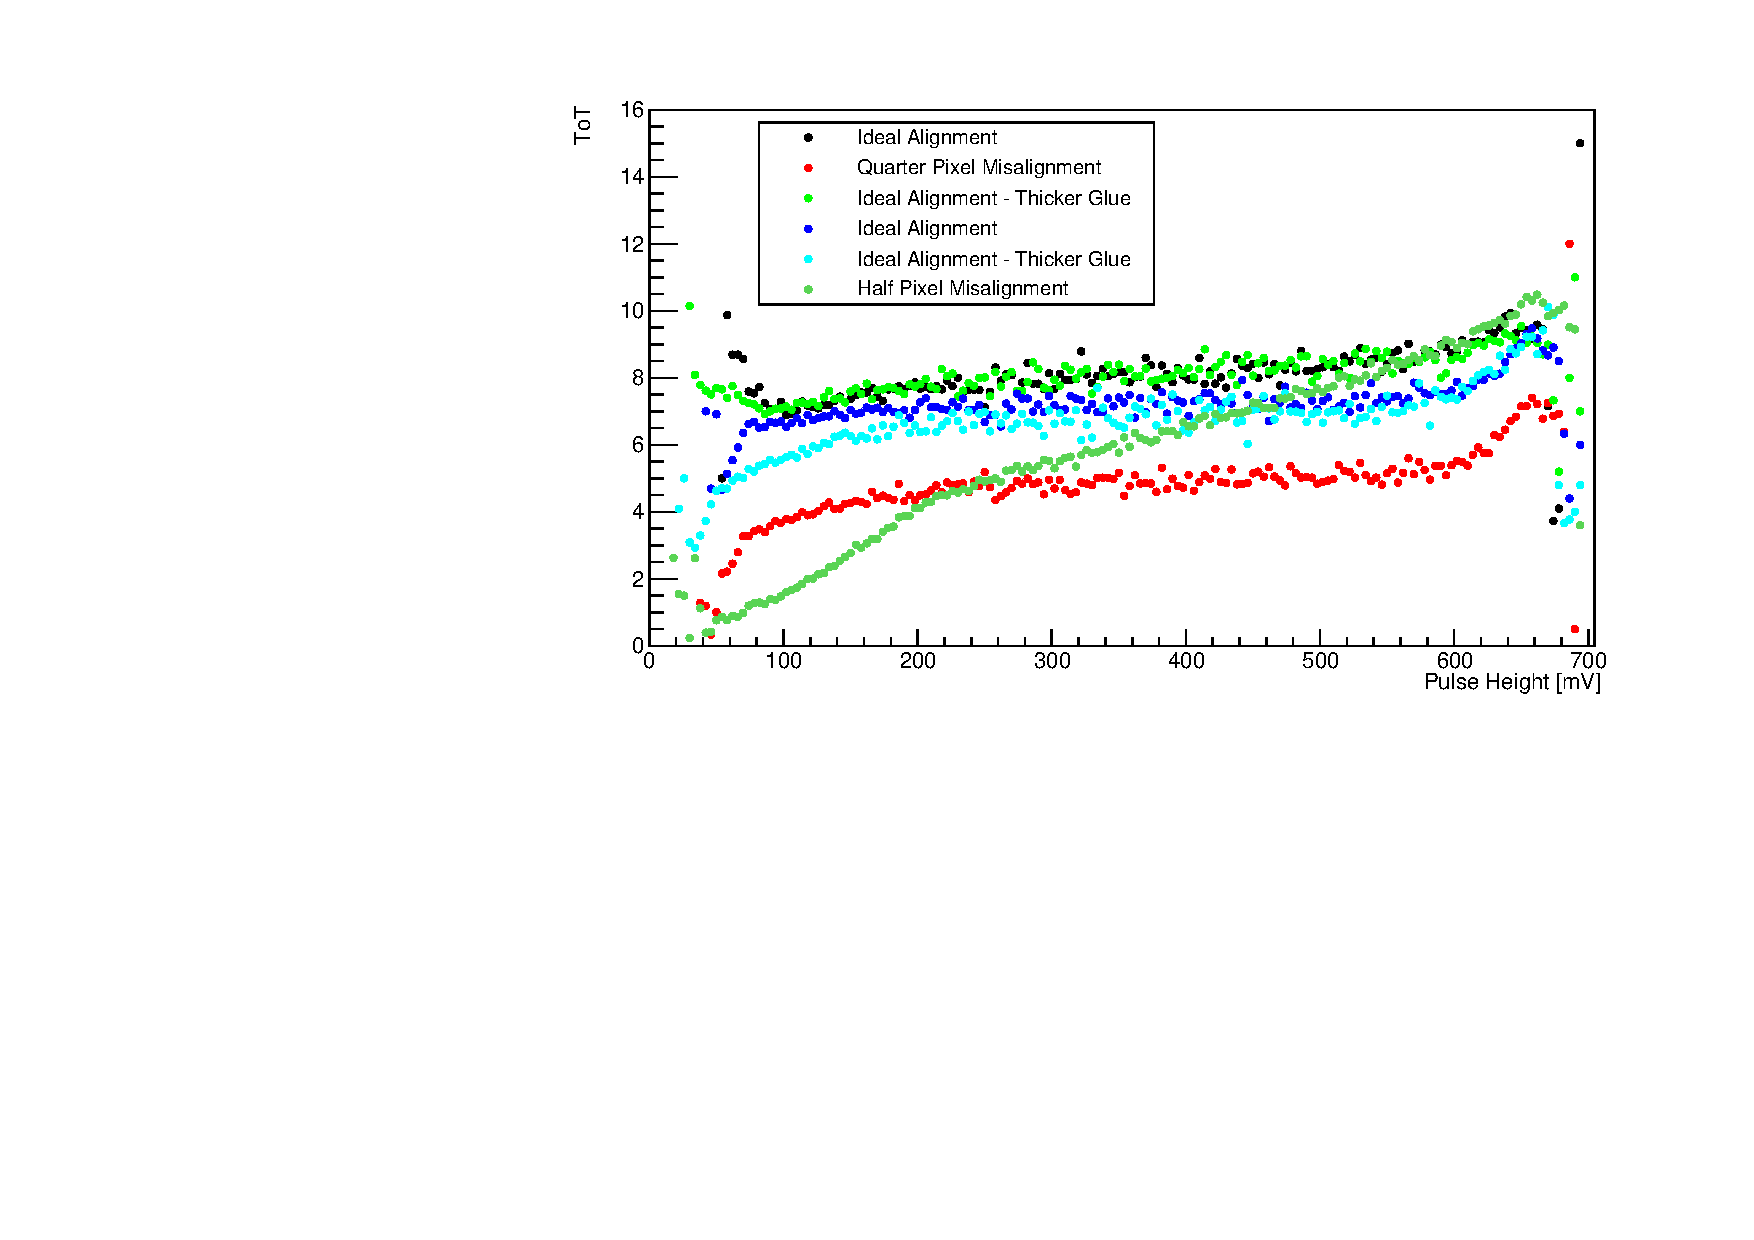
\includegraphics[width=0.5\textwidth]{CLICdpVertex/Plots/ToT_X_vs_PulseHeight.pdf}
\caption[Average ToT on adjacent pixel vs pulse height.]{Average ToT on adjacent pixel vs pulse height.}
\label{fig:avgtotadjvspulseheight}
\end{figure}

\subsection{Test Pulse Calibration}
Inject pulse height of fixed size directly into CLICPix and recored ToT.  This cannot be done for the HV-CMOS due to the device construction preventing getting to the relevant input to the HV-CMOS.  Plots of average ToT vs pulse height, describe surrogate function fit and column structure.  

\section{Test Beam Analysis}
\subsection{Test Beam Area}
Description of test beam, site and telescope.

\subsection{Efficiency}

\begin{itemize}
\item Description of masks and why they need to be applied.
\item Alignment description.
\item Efficiency calculations and conclusions. 
\end{itemize}

\begin{figure}
\centering
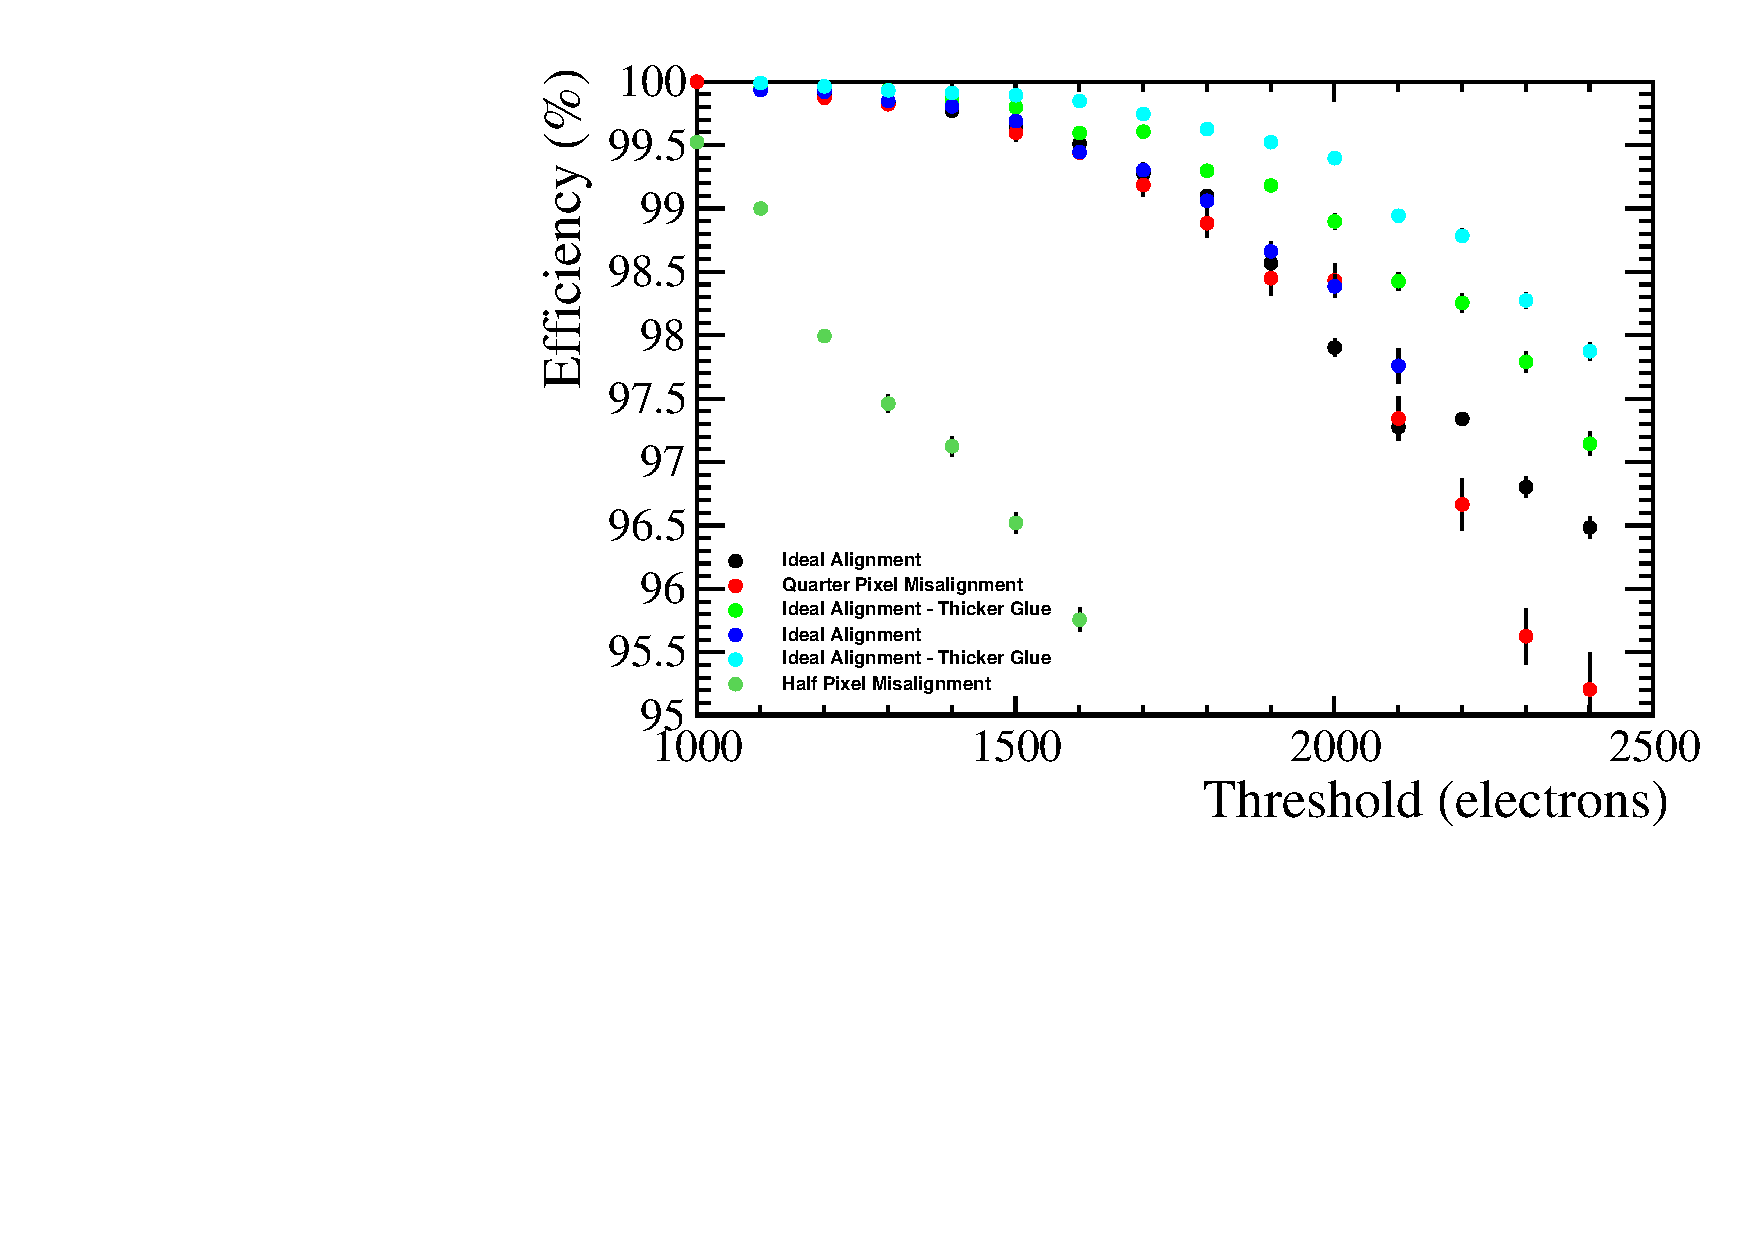
\includegraphics[width=0.5\textwidth]{CLICdpVertex/Plots/ZoomedEfficiency.pdf}
\caption[Efficiency vs threshold.]{Efficiency vs threshold.}
\label{fig:efficiency}
\end{figure}




  
